\documentclass[a4paper]{article}

\usepackage[LGR]{fontenc}
\usepackage{titling}
\usepackage[greek]{babel}
\usepackage{amsmath}
\usepackage{mathtools}
\usepackage{breqn}
\usepackage{hyperref}
\usepackage{graphicx}
\graphicspath{ {../Euler/}, {../ImprovedEuler/}, {../Problem_1_3/}, {../problem2d/} }
\hypersetup{
    colorlinks,
    citecolor=black,
    filecolor=black,
    linkcolor=black,
    urlcolor=black
}




%------------------------------------------------------------------------------------------------
% basic info (date, title etc...)
%------------------------------------------------------------------------------------------------
\author{Παύλος Ορφανίδης: 4134 \and Γιώργος Χατζηλίγος: 4835 \and Σπύρος Κοντάκης: 4702}
\date{\today}
\title{Υπολογιστικά Μαθηματικά 2021--2022}

%------------------------------------------------------------------------------------------------
% Adding the option to append a number next to equations
%------------------------------------------------------------------------------------------------
\newcommand{\dd}[1]{\mathrm{d}#1}

\begin{document}
%------------------------------------------------------------------------------------------------
% Creating the title and the contents page
%------------------------------------------------------------------------------------------------
    \maketitle
    \tableofcontents

%------------------------------------------------------------------------------------------------
% Creating a first section that includes general data given by the instructor
%------------------------------------------------------------------------------------------------

    \section*{Γενικά δεδομένα}
        \begin{equation}
            AM = 4835
        \end{equation}
        \begin{equation}
            ms'' = (f_1+f_2)-b_s\rvert s' \lvert s'
        \end{equation}
        \begin{equation}
            I_z\omega '=\frac{d}{2}(f_2-f_1)-b_{\theta}\rvert\omega\lvert\omega
        \end{equation}
        \begin{equation}
            s(0)=s_0
        \end{equation}
        \begin{equation}
            s'(0)=0,\quad \omega(0)=0
        \end{equation}
        \[m=9kg\]
        \[d=1m\]
        \[I_z=0.38 kgm^2\]
%------------------------------------------------------------------------------------------------
% Excersise 1
%------------------------------------------------------------------------------------------------
    \section{Πρόβλημα 1}
        \subsection*{Μεταφορική κίνηση}
        \subsubsection*{$Euler$ $s'$}
        Έχουμε από τα δεδομένα ότι:
        \begin{equation}
            s''=f'(t,s')=(f1+f2)-bs|s'|s'
        \end{equation}
        \begin{equation}
            s'=f(t,s)
        \end{equation}
        \[{[f_1,f_2]}^T={[A.M./7000, A.M./7000]}^T\]
        \[{[f_1,f_2]}^T={[A.M./7000, A.M./8000]}^T\]
        \[s_0=\frac{A.M.}{1000}\]
        \[\theta_0=0\]

        
            \begin{tabular}{ll}
                Εφαρμόζουμε την μέθοδο $Euler$:                             &                               \\
                $t_n=t_0+nh$                                                & $s'_{n+1}=s'_n+hf'(t,s')_n$   \\
                το οποίο σημαίνει ότι:                                      & $s'_1=s'_0+hs''_0$            \\
                $t_1=t_0+1h$                                                & $s'_2=s'_1+hs''_1$            \\
                $t_2=t_0+2h$                                                & .                             \\
                .                                                           & .                             \\
                .                                                           & .                             \\
                .                                                           &                               \\
                $t_n=t_0+nh$                                                &                         
            \end{tabular}

            \subsubsection*{$Euler$ $s$}
            \begin{tabular}{ll}
                Εφαρμόζουμε την μέθοδο $Euler$:                             &                               \\
                $t_n=t_0+nh$                                                & $s_{n+1}=s_n+hs'_n$   \\
                το οποίο σημαίνει ότι:                                      & $s_1=s_0+hs'_0$            \\
                $t_1=t_0+1h$                                                & $s_2=s_1+hs'_1$            \\
                $t_2=t_0+2h$                                                & .                             \\
                .                                                           & .                             \\
                .                                                           & .                             \\
                .                                                           &                               \\
                $t_n=t_0+nh$                                                &                         
            \end{tabular}
            \subsection*{Στροφική κίνηση}
            
            \begin{equation}
                \omega'=\frac{\frac{d}{2}(f_2-f_1)-b\theta\rvert\omega\lvert\omega}{I_z}=f(t,\omega)
            \end{equation}
            \subsubsection*{$Euler$}
            \begin{tabular}{ll}
                $t_{n+1}=t_0+nh$ & $\omega_{n+1} = \omega_0+h\omega'h$\\
                $t_1 = t_0+1h$&$\omega_1 = \omega_0+h\omega'_0$\\
                $t_2=t_0+2h$ & $\omega_2=\omega_1+h\omega'_1$\\
                .&.\\
                .&.\\
                .&.\\
                $t_{30.000}=t_0+29.999h$&$\omega_{30.000}=\omega_{29.999}+h\omega'_{29.999}$\\
            \end{tabular}

        \subsubsection*{Bελτιωμένη μέθοδος $Euler$ $s'$}

        \begin{tabular}{l|l}
            \multicolumn{2}{c}{Εφαρμόζουμε την βελτιωμένη μέθοδο $Euler$: }\\
            $t_n=t_0+nh$ & $s'_{n+1}=s'_n+\frac{h}{2}{[f'(t_n,s_n+s'_n, s'_n)+f'(t_n+h, s'_n+hf'(t_n,s'_n))]}$\\
            το οποίο σημαίνει ότι:& $s'_{n+1}=s'_{n}+\frac{h}{2}[s''(n)+\frac{f_1+f_2}{m}-\frac{(b_s\rvert s'_n+hs''_n\lvert(s'_n+hs''_n))}{m}]$\\
            $t_1=t_0+1h$          &το οποίο σημαίνει ότι: \\
            $t_2=t_0+2h$          & $s'_1=s'_0+\frac{h}{2}{[s''_0+\frac{f_1+f_2}{m}+\frac{\lvert b_ss'_0+hs''_0\rvert(b_ss'_0+hs''_0)}{m}]}$\\
            .                     & .\\
            .                     & .\\
            .                     & .\\
            $t_n=t_0+nh$          &  \\
        \end{tabular}
        
        
      %--------------------------------------------------------------------  
        % Changes required
      %--------------------------------------------------------------------
        \subsubsection*{Bελτιωμένη μέθοδος $Euler$ $s$}
        H peplegm'enh morf'h pou mas bohj'a kai ja efarm'osoume e'inai:

        \begin{tabular}{l|l}
            \multicolumn{2}{c}{Εφαρμόζουμε την βελτιωμένη μέθοδο $Euler$: }\\
            $t_n=t_0+nh$ & $s_{n+1}=s_n+\frac{h}{2}[s'_n+s'_{n+1}]$\\
            το οποίο σημαίνει ότι:& $s_1=s_0+\frac{h}{2}[s'_0+s'_1]$\\
            $t_1=t_0+1h$          &$s_2=s_1+\frac{h}{2}[s'_1+s'_2]$ \\
            $t_2=t_0+2h$          & .\\
            .                     & .\\
            .                     & .\\
            .                     & .\\
            $t_n=t_0+nh$          &  \\
        \end{tabular}
        
        
        \subsection*{Στροφική κίνηση}

        \begin{dmath}
            \omega_{n+1}=\omega_n+\frac{h}{2}{[f(t, \omega)+f(t_n+h, \omega_n+f(t,\omega))]}=\omega_n+\frac{h}{2}{[\omega'_n+\frac{(\frac{d}{2}(f_2-f_1)-b\theta \lvert\omega_n+\omega'_n\rvert(\omega_n+\omega'_n))}{I_z}]}
        \end{dmath}
%------------------------------------------------------------------------------------------------
% Excersise 1γ
%------------------------------------------------------------------------------------------------
        \subsection{Eρώτημα γ: Μέθοδος $Euler$}

        \subsubsection{Δεδομένα:}
            \[f_1 + f_2 = K_{ps} (s_{des} - s) - K_{ds}(s')\]
            \[K_{ps} = 5\]
            \[K_{ds} = 15 + \frac{AM}{100}\]
            \[S_0 =0\]
            \[S_{des} = \frac{AM}{200}\]

        \subsection{Μεταφορική Κίνηση}
        \subsection{M'ejodos $Euler$}
        \begin{equation}
            f_1+f_2=K_{ps}(s_{des}-s)-K_{ds}s'
            \label{2}
        \end{equation}

        εφόσων ξέρω τον τύπο:

        \begin{equation}
            s''=\frac{f_1+f_2-b_s\rvert s'\lvert s'}{m}
            \label{1}
        \end{equation}

        \[(\ref{1}) \xRightarrow{(\ref{2})}s''=\frac{k_{ps}(s_{des}-s)-K_{ds}s'-b_s\rvert s'\lvert s'}{m}=f(t,s,s')\]

        
        \begin{tabular}{l|l}
            \multicolumn{2}{c}{Εφαρμόζουμε $Euler$ για την $s'$: }\\
            $t_n=t_0+nh$ & $s'_{n+1}=s'_n+hs''_n$\\
            το οποίο σημαίνει ότι: & \\
            $t_1=t_0+1h$ & $s'_1=s'_0+hs''_0$\\
            $t_2=t_0+2h$ & $s'_2=s'_1+hs''_1$(Dιότι έχει άγνωστη $s_1$)\\
            .            & $s'_3=s'_2+hs''_2$(Dιότι έχει άγνωστη $s_2$)\\
            . & \\
            . & \\
            $t_n=t_0+nh$ & \\
        \end{tabular} 
        %--------------------------------------------
        %  Arrows to point between functions
        %--------------------------------------------
        
        \begin{tabular}{l|l}
            \multicolumn{2}{c}{Εφαρμόζουμε $Euler$ για την $s$: }\\
            $t_n=t_0+nh$ & $s_{n+1}=s_n+hs'_n$\\
            το οποίο σημαίνει ότι: & \\
            $t_1=t_0+1h$ & $s_1=s_0+hs'_0$\\
            $t_2=t_0+2h$ & $s_2=s_1+hs'_1$\\
            .            &\\
            . & \\
            . & \\
            $t_n=t_0+nh$ & \\
        \end{tabular}
% Βελτιωμένη μέθοδος Euler



        \subsection{Πρόβλημα 1γ: Βελτιωμένη Μέθοδος $Euler$}

        \subsubsection{Δεδομένα}

        \[f_1 + f_2 = K_{ps}(s_{des} - s) - K_{ds}(s')\]
        \[K_{ps} = 5\]
        \[K_{ds} = 15 + (AM/ 100)\]
        \[S_0 =0\]
        \[S_{des} = AM / 200\]
        \[s''=\frac{k_{ps}(s_{des}-s)-k_{ds}s'-b_s\lvert s'\rvert s'}{m}=f'(t,s,s')\]
        \[s'=f(t,s)\]
        \subsubsection{Μεταφορική Κίνηση}   
        Για την $s'(t)$:

        \begin{tabular}{ll}
            $t_n = t_0 + nh$		&	$s'_{n+1}=s'_n+\frac{h}{2}[f'(t,s,s')+f'(t_n+h, s_n+f(t_n, s), s'_n+f'(t,s,s'))]$\\
            $t_1 = t_0  + 1h$		&	$s'_{n+1}=s'_n+\frac{h}{2}[s''_n+\frac{(k_{ps}(s_{des}-(s_n+hs'_n))-k_{ds}(s'_n+hs''_n)-b_s\lvert s'_n+h''_n\rvert(s'_n+h''_n))}{m}]$\\
            $t_2 = t_0  + 2h$		&	$s'_{1}=s'_0+\frac{h}{2}[s''_0+\frac{(k_{ps}(s_{des}-(s_0+hs'_0))-k_{ds}(s'_0+hs''_0)-b_s\lvert s'_0+h''_0\rvert(s'_0+h''_0))}{m}]$\\
            \multicolumn{2}{c}{.}\\
            \multicolumn{2}{c}{.}\\
            \multicolumn{2}{c}{.}\\
            $t_{30.000} = t_0 + 30.000h$&
        \end{tabular}

        \vspace{70pt}

        \begin{tabular}{l|l}
            \multicolumn{2}{c}{Εφαρμόζουμε την βελτιωμένη μέθοδο $Euler$: }\\
            $t_n=t_0+nh$ & $s_{n+1}=s_n+\frac{h}{2}[s'_n+s'_{n+1}]$\\
            το οποίο σημαίνει ότι:& $s_1=s_0+\frac{h}{2}[s'_0+s'_1]$\\
            $t_1=t_0+1h$          &$s_2=s_1+\frac{h}{2}[s'_1+s'_2]$ \\
            $t_2=t_0+2h$          & .\\
            .                     & .\\
            .                     & .\\
            .                     & .\\
            $t_n=t_0+nh$          &  \\
        \end{tabular}
%-------------------------------------------------------------------------
% Images
%-------------------------------------------------------------------------
        \subsection{Grafik'es parast'aseis}
        \subsubsection*{1a) $Euler$}
        \noindent\makebox[\textwidth]{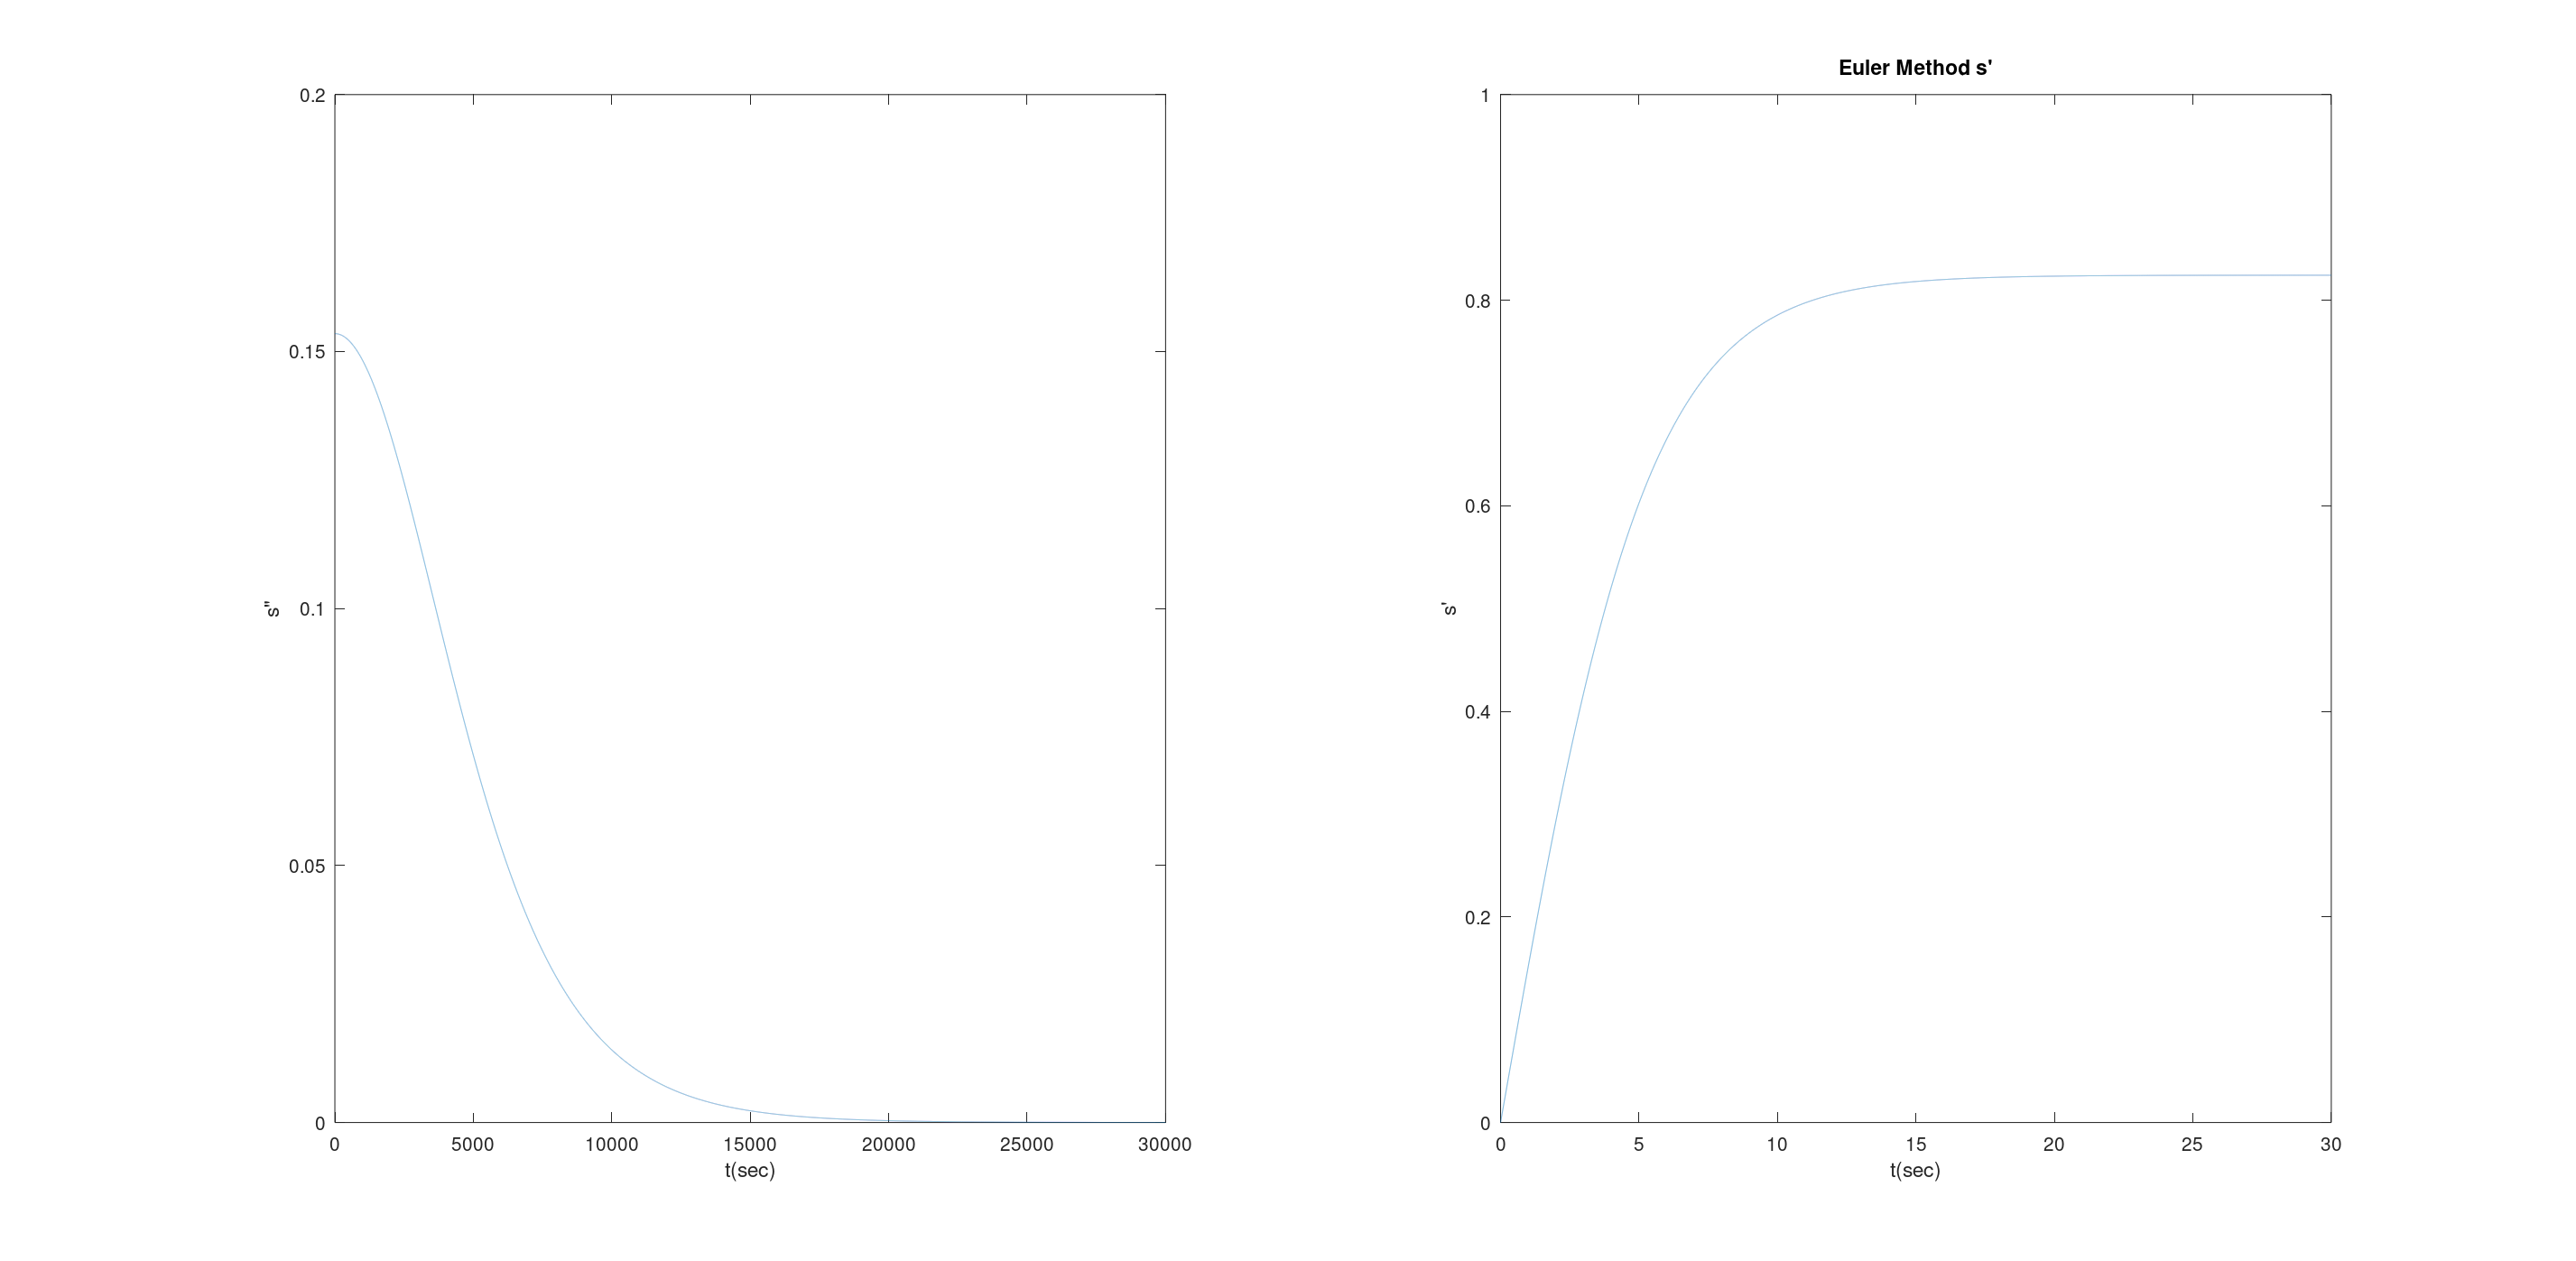
\includegraphics[width=\paperwidth]{Euler1.png}}
        \noindent\makebox[\textwidth]{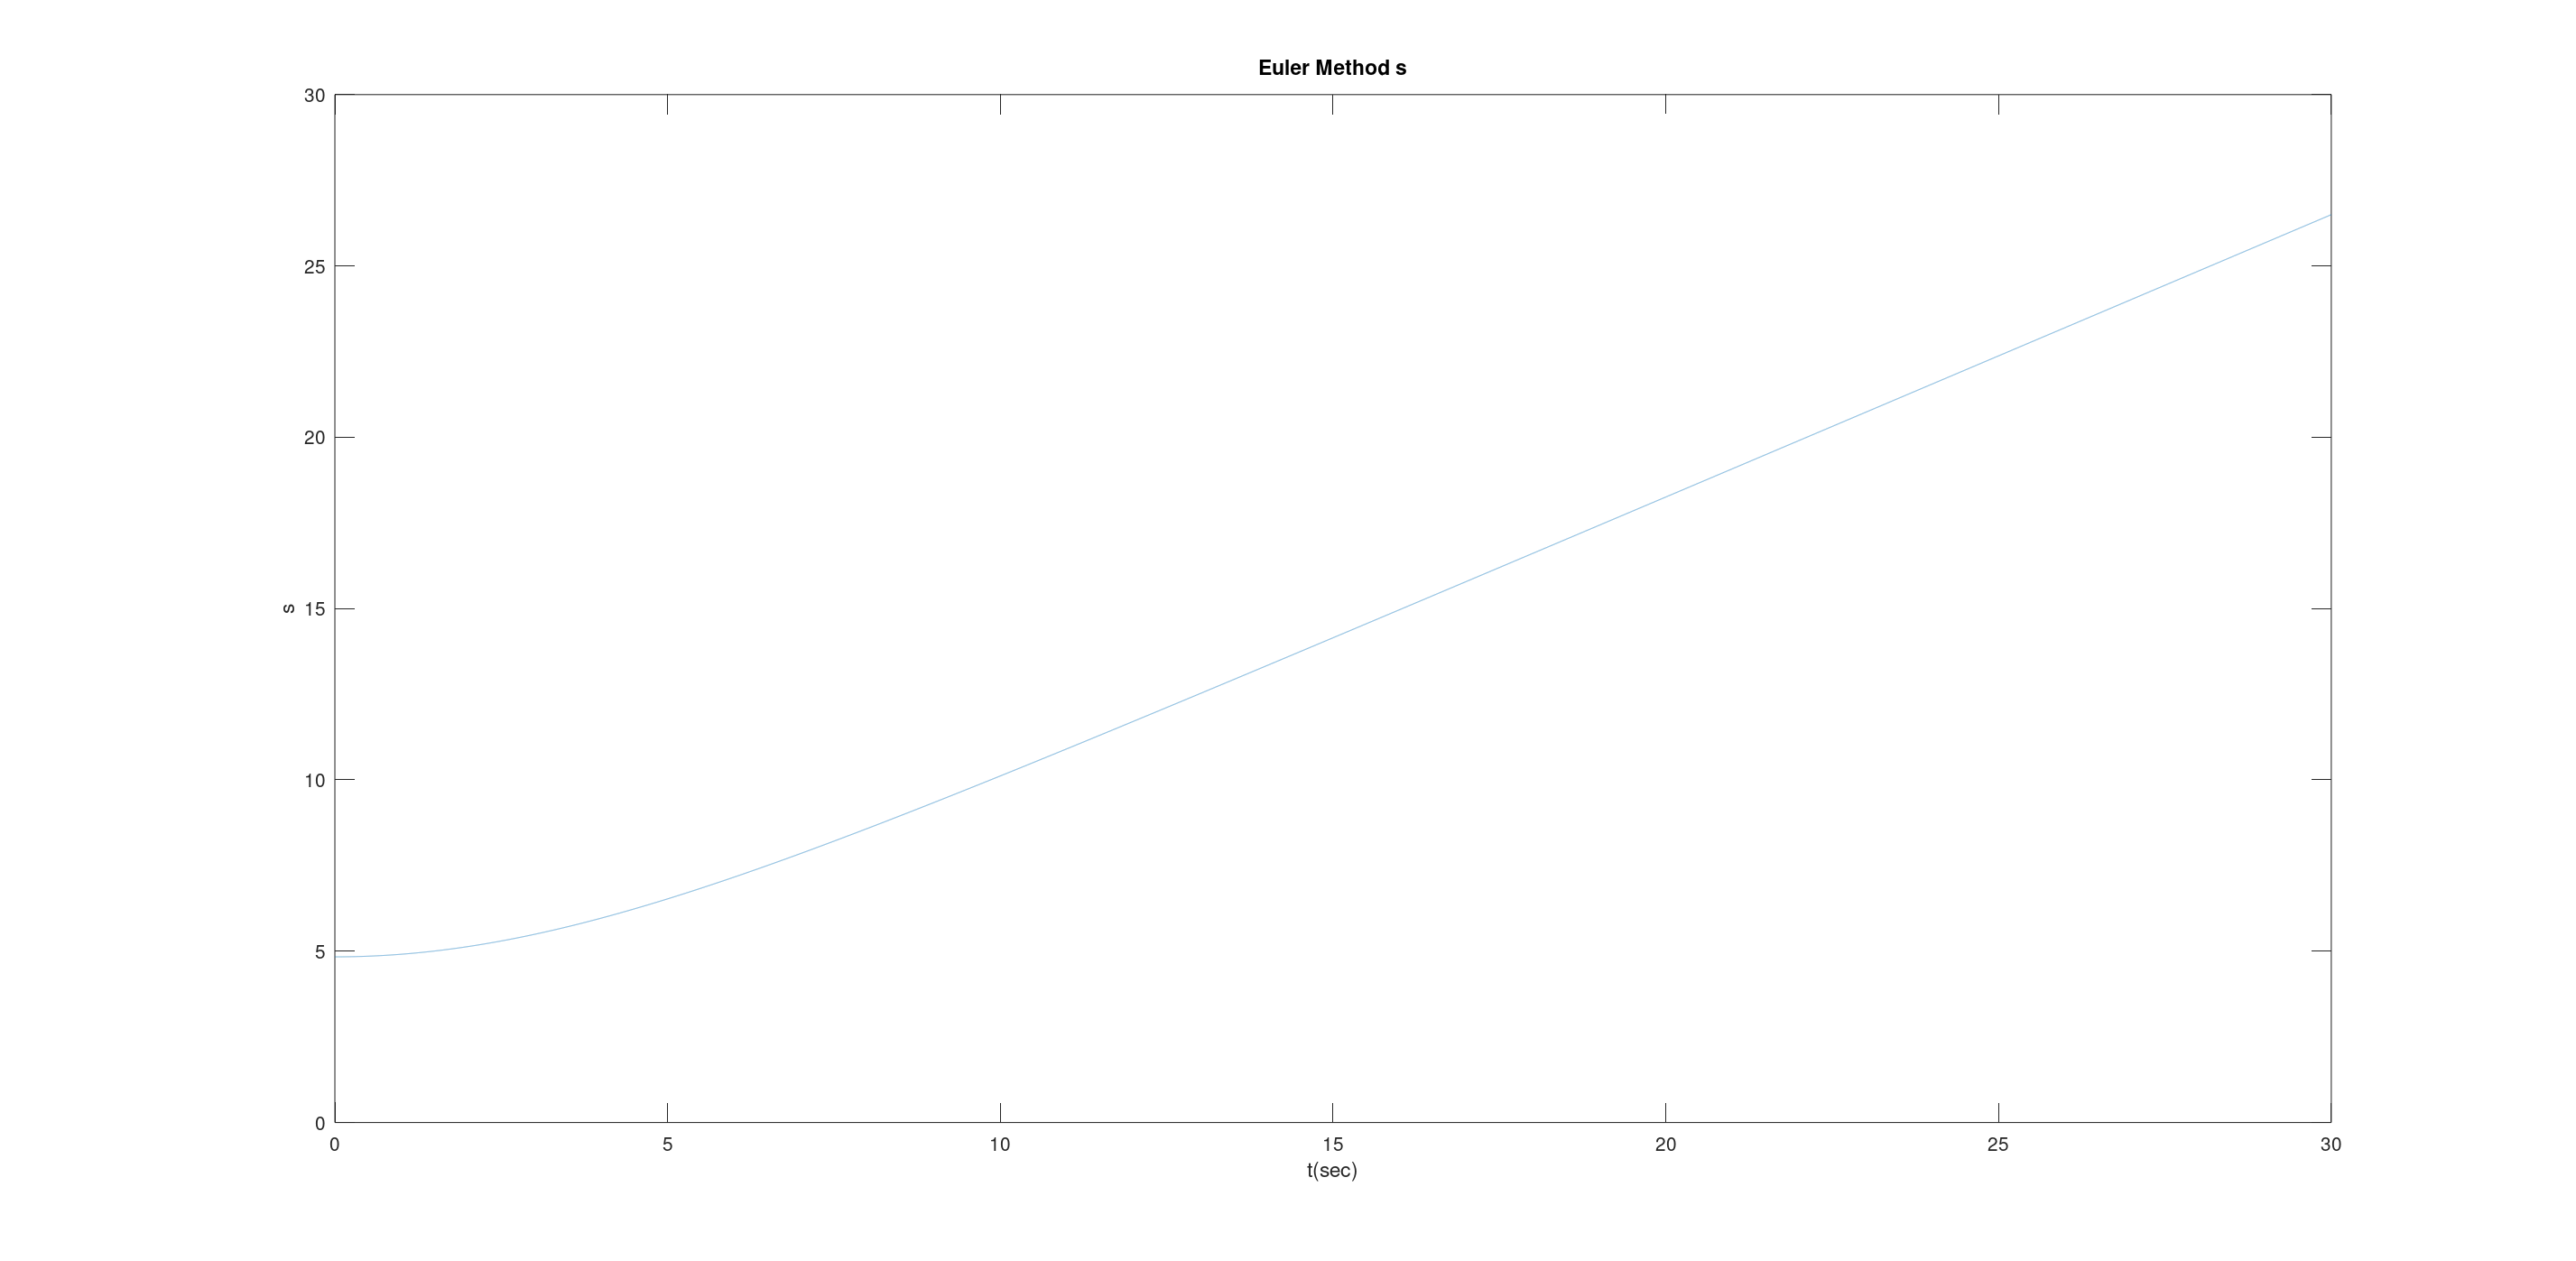
\includegraphics[width=\paperwidth]{Euler2.png}}
        \noindent\makebox[\textwidth]{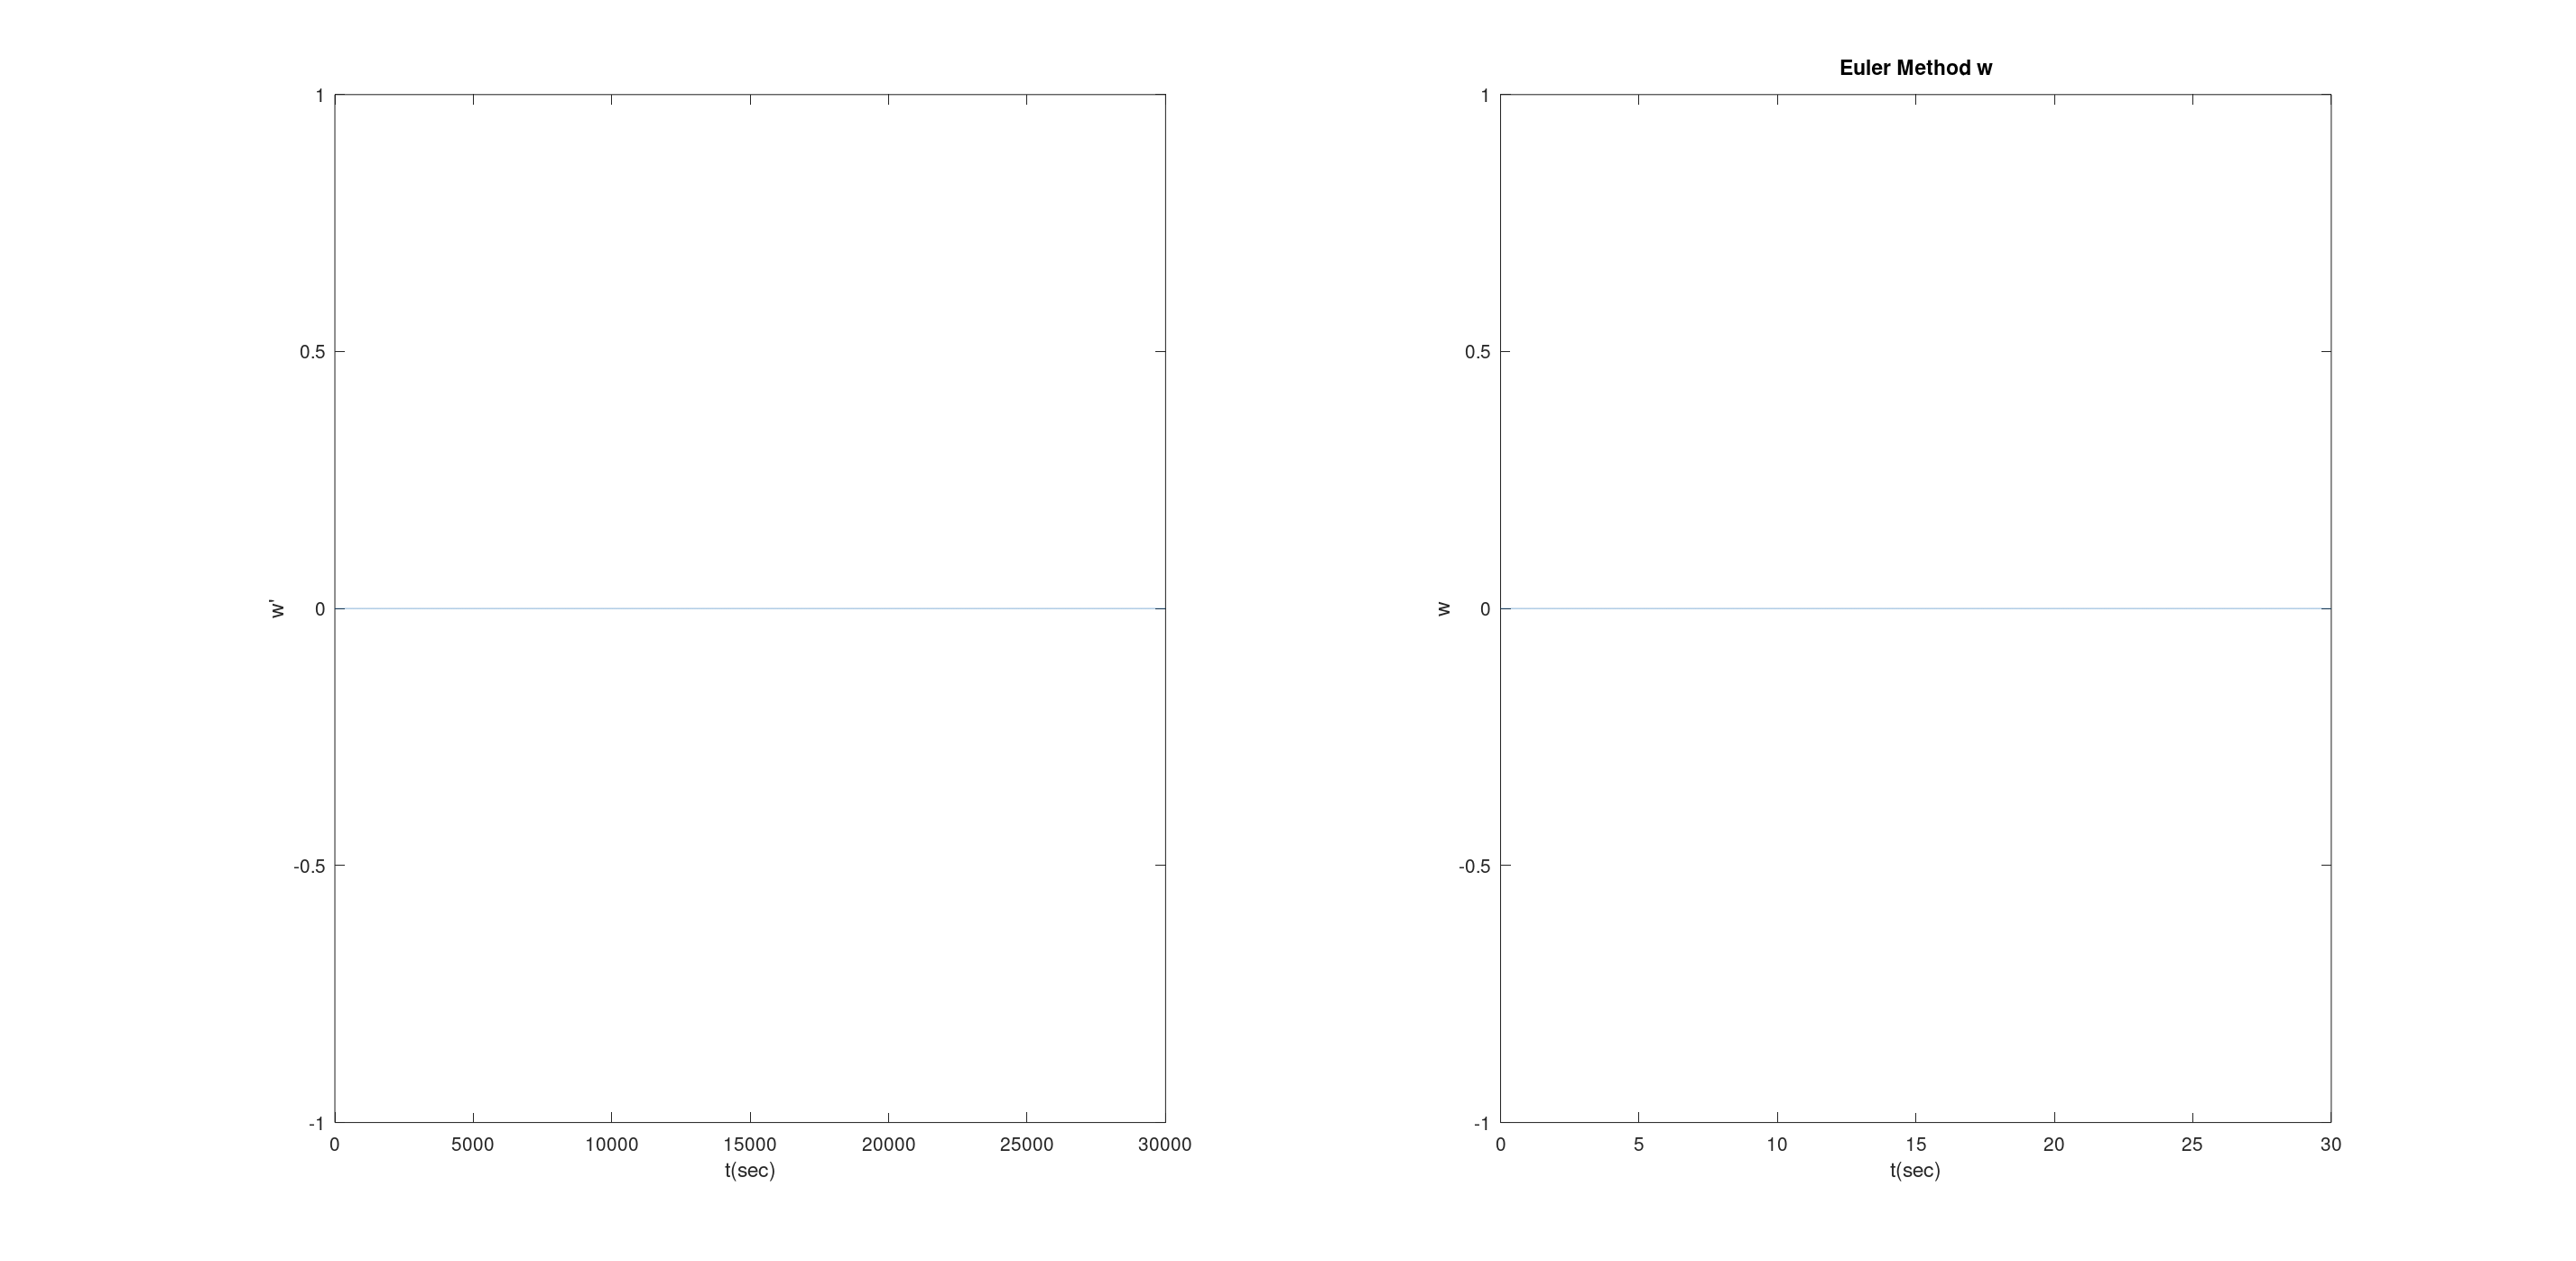
\includegraphics[width=\paperwidth]{Euler3.png}}
        \noindent\makebox[\textwidth]{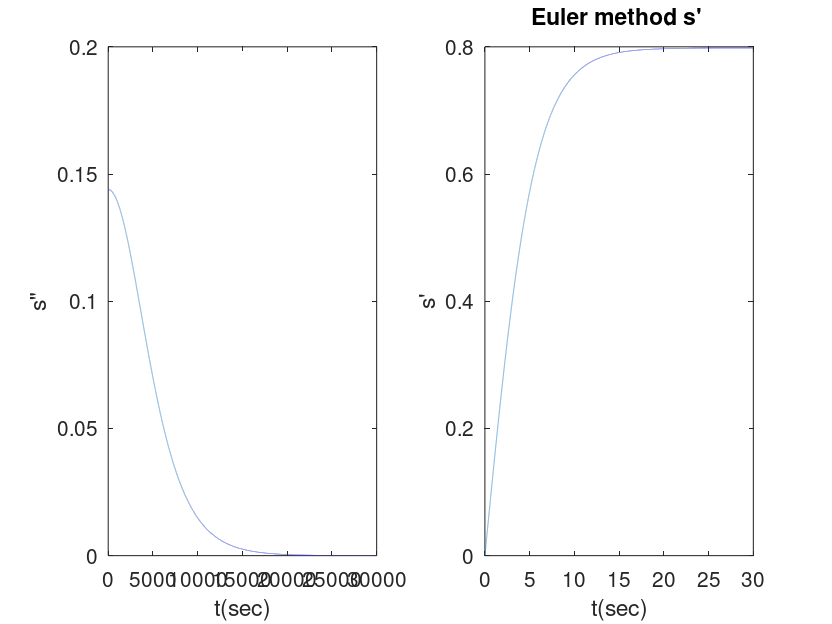
\includegraphics[width=\paperwidth]{Euler4.png}}
        \noindent\makebox[\textwidth]{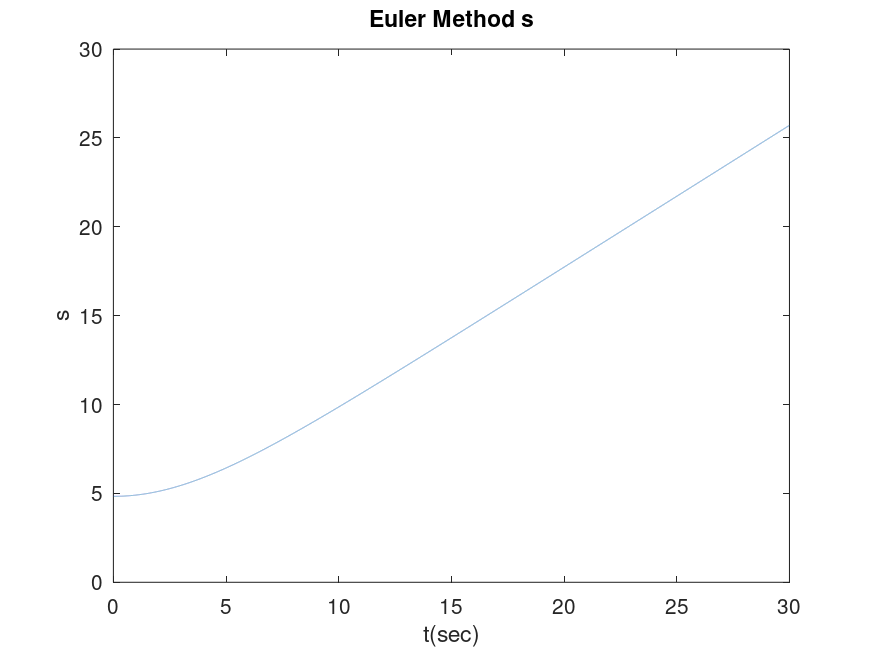
\includegraphics[width=\paperwidth]{Euler5.png}}
        \noindent\makebox[\textwidth]{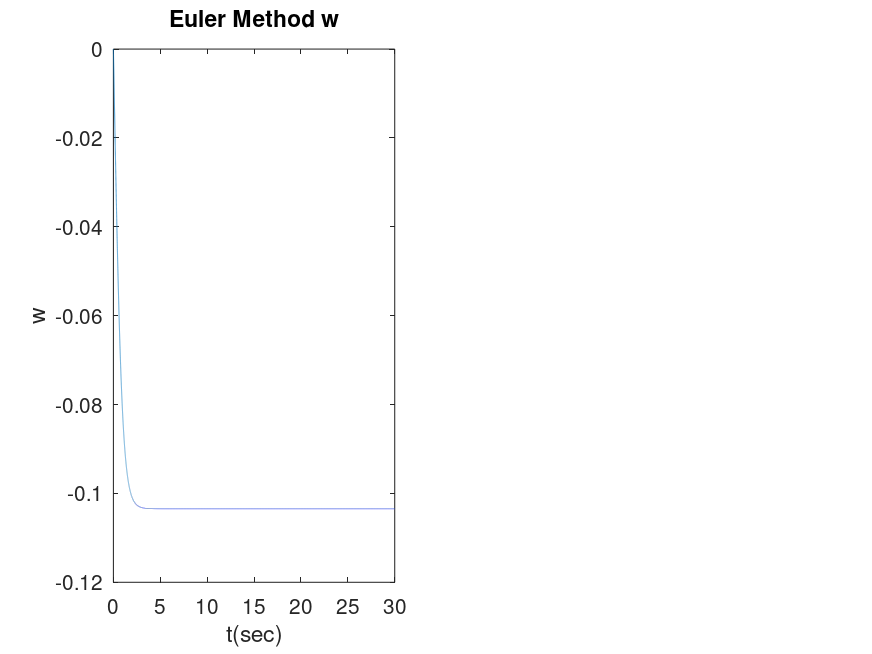
\includegraphics[width=\paperwidth]{Euler6.png}}
        \subsubsection*{1a) Beltiwm'enh $Euler$}
        \noindent\makebox[\textwidth]{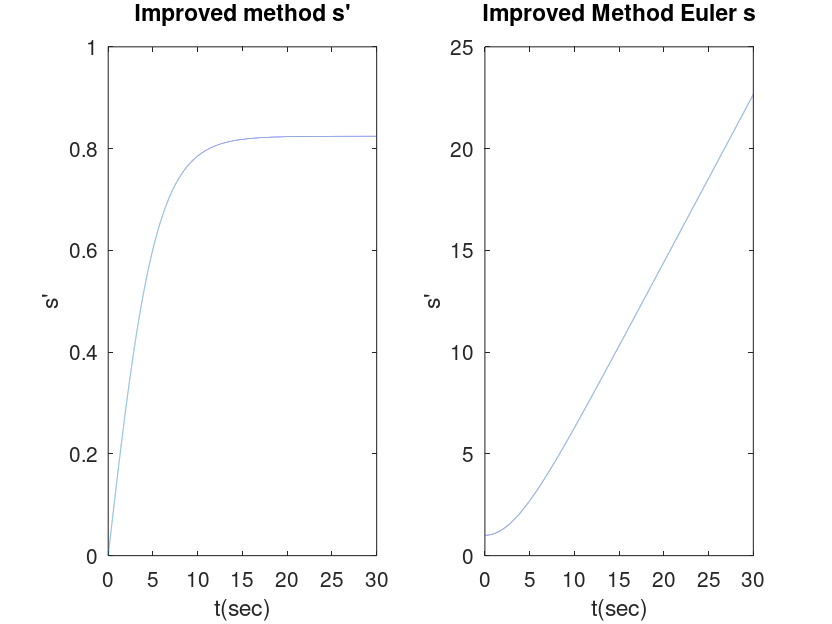
\includegraphics[width=\paperwidth]{ImprovedEuler1.png}}
        
        \noindent\makebox[\textwidth]{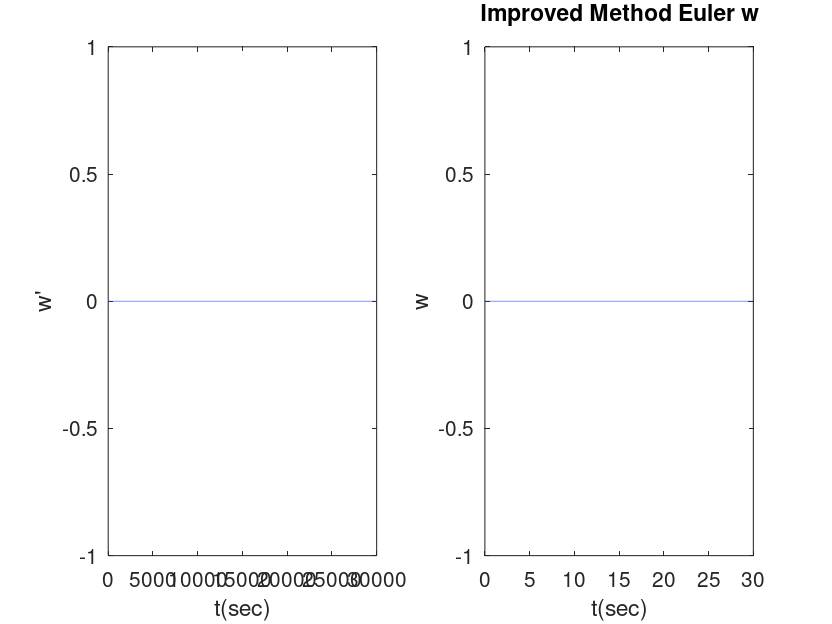
\includegraphics[width=\paperwidth]{ImprovedEuler2.png}}
        \noindent\makebox[\textwidth]{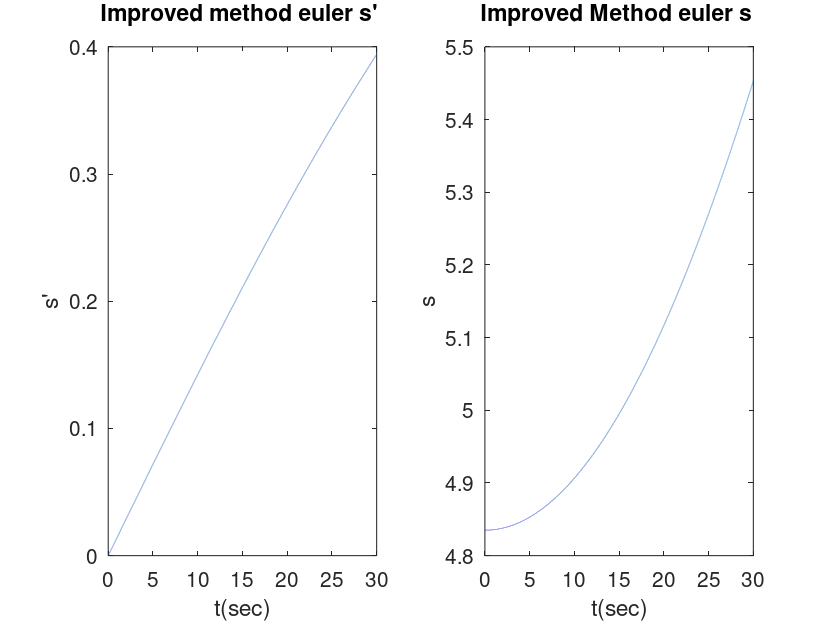
\includegraphics[width=\paperwidth]{ImprovedEuler3.png}}
        \noindent\makebox[\textwidth]{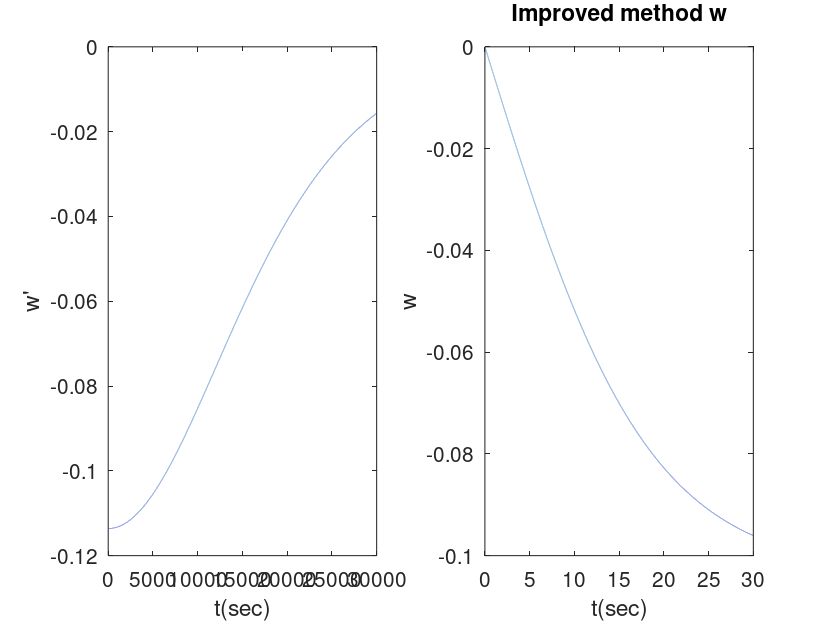
\includegraphics[width=\paperwidth]{ImprovedEuler4.png}}

        \subsubsection*{1g) $Euler$ kai beltiwm'enh}
        \noindent\makebox[\textwidth]{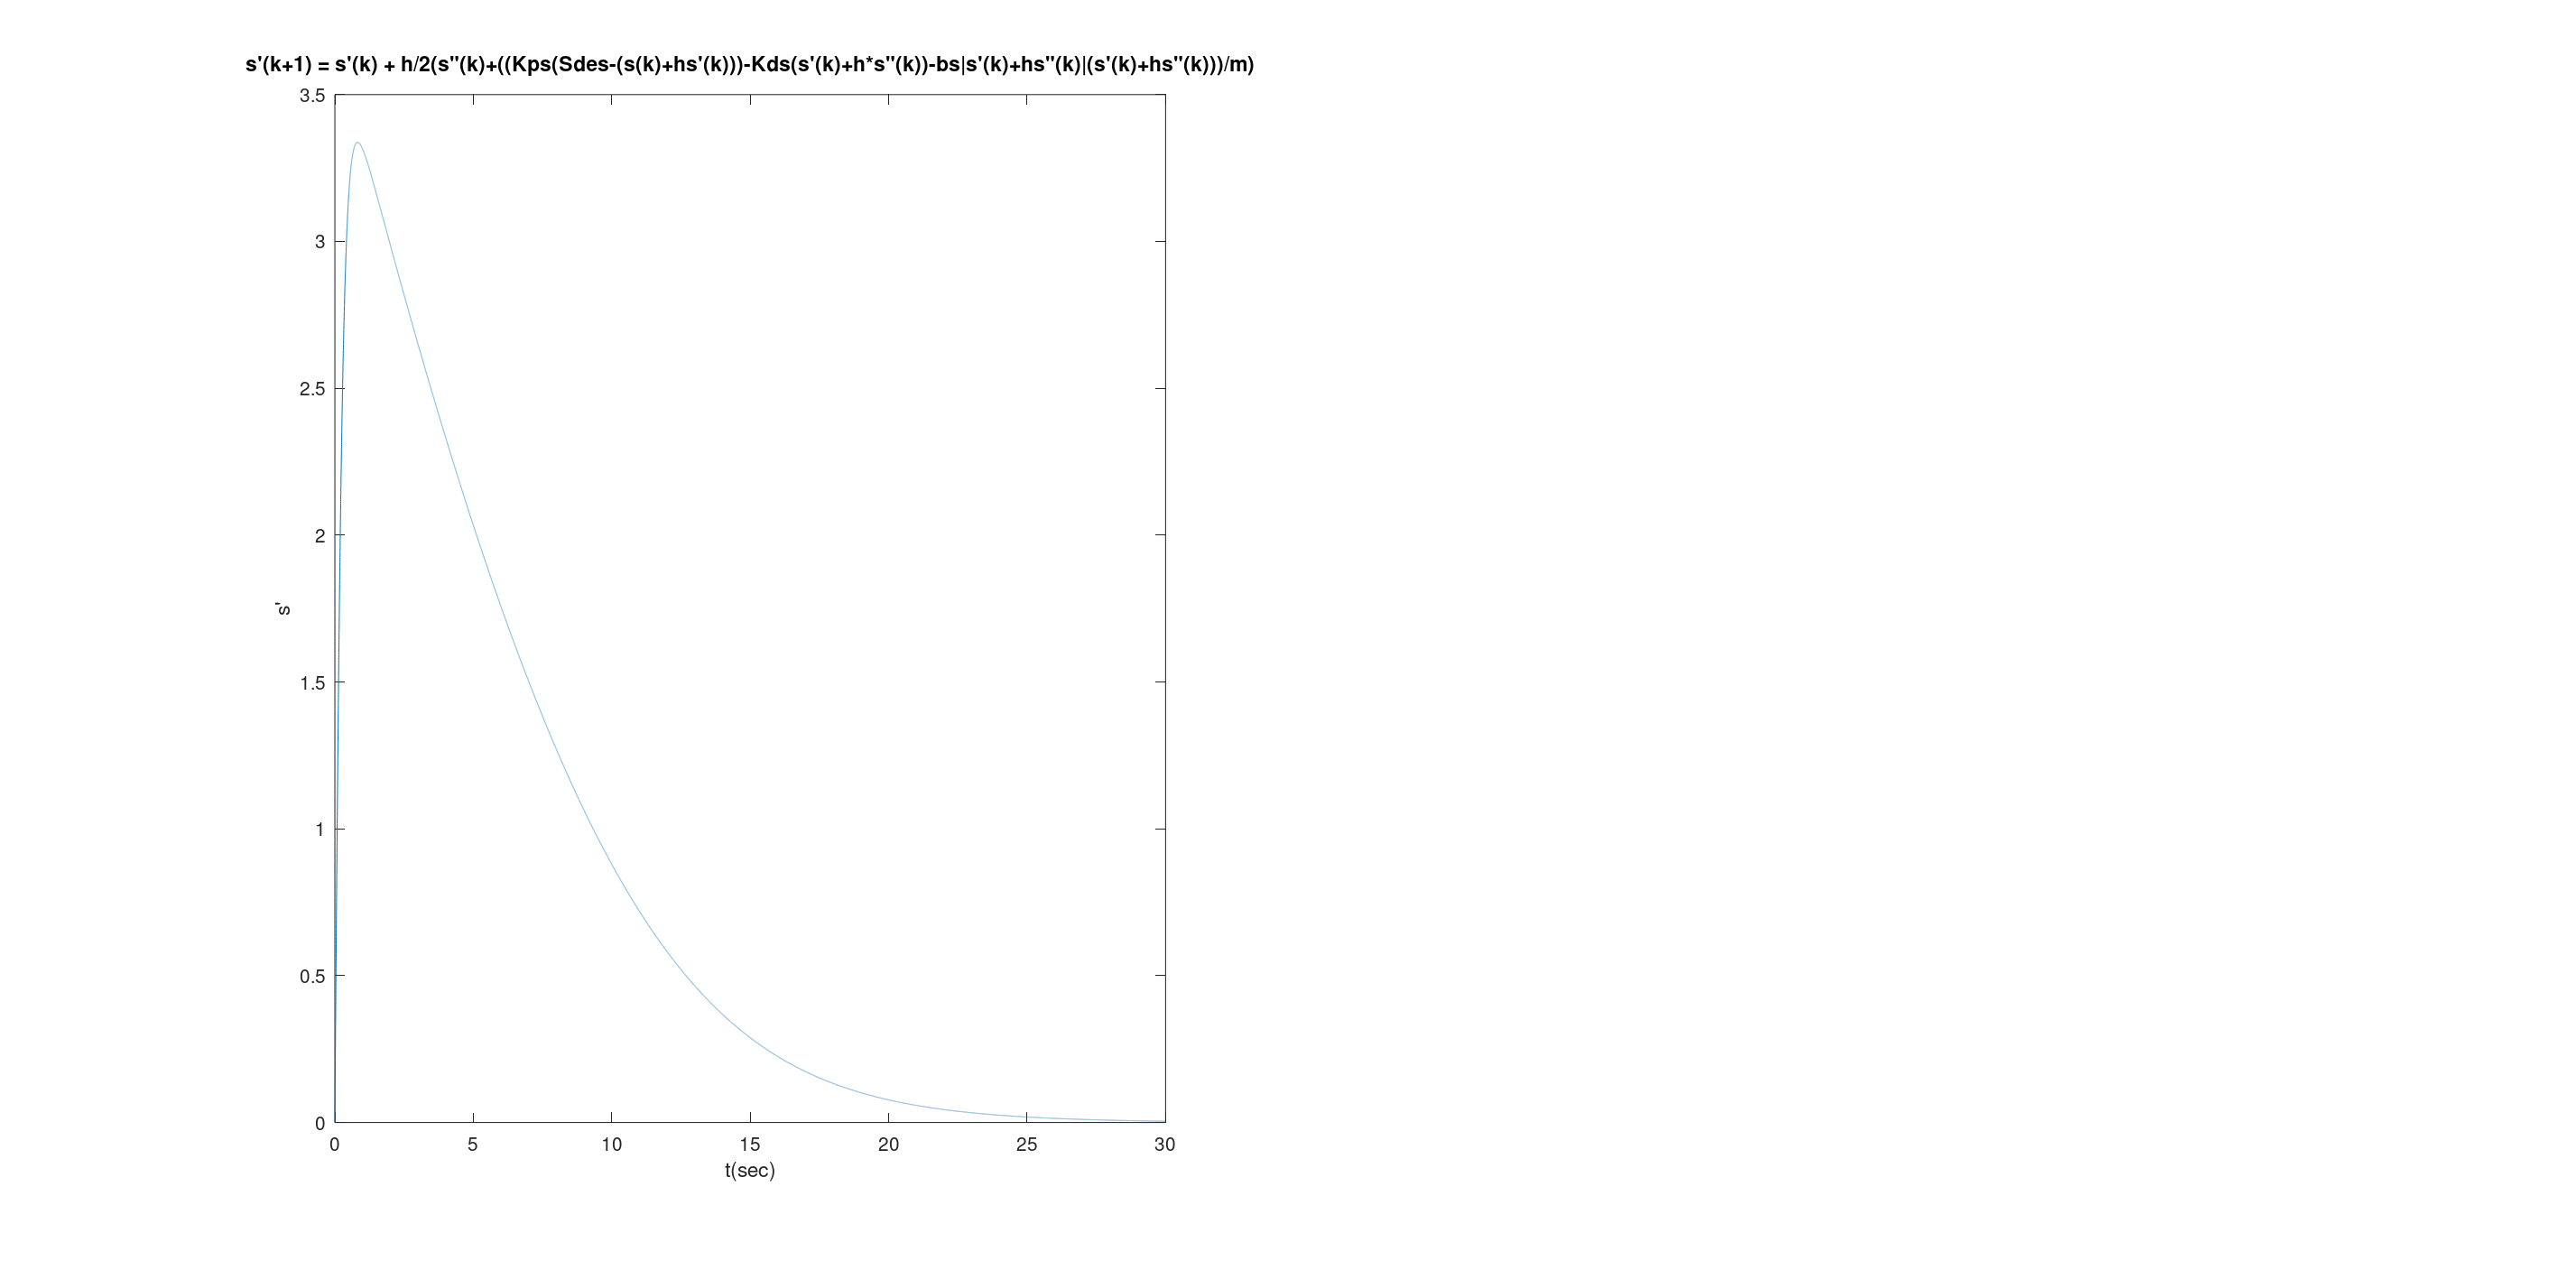
\includegraphics[width=\paperwidth]{problem_1_3_1}}
        \noindent\makebox[\textwidth]{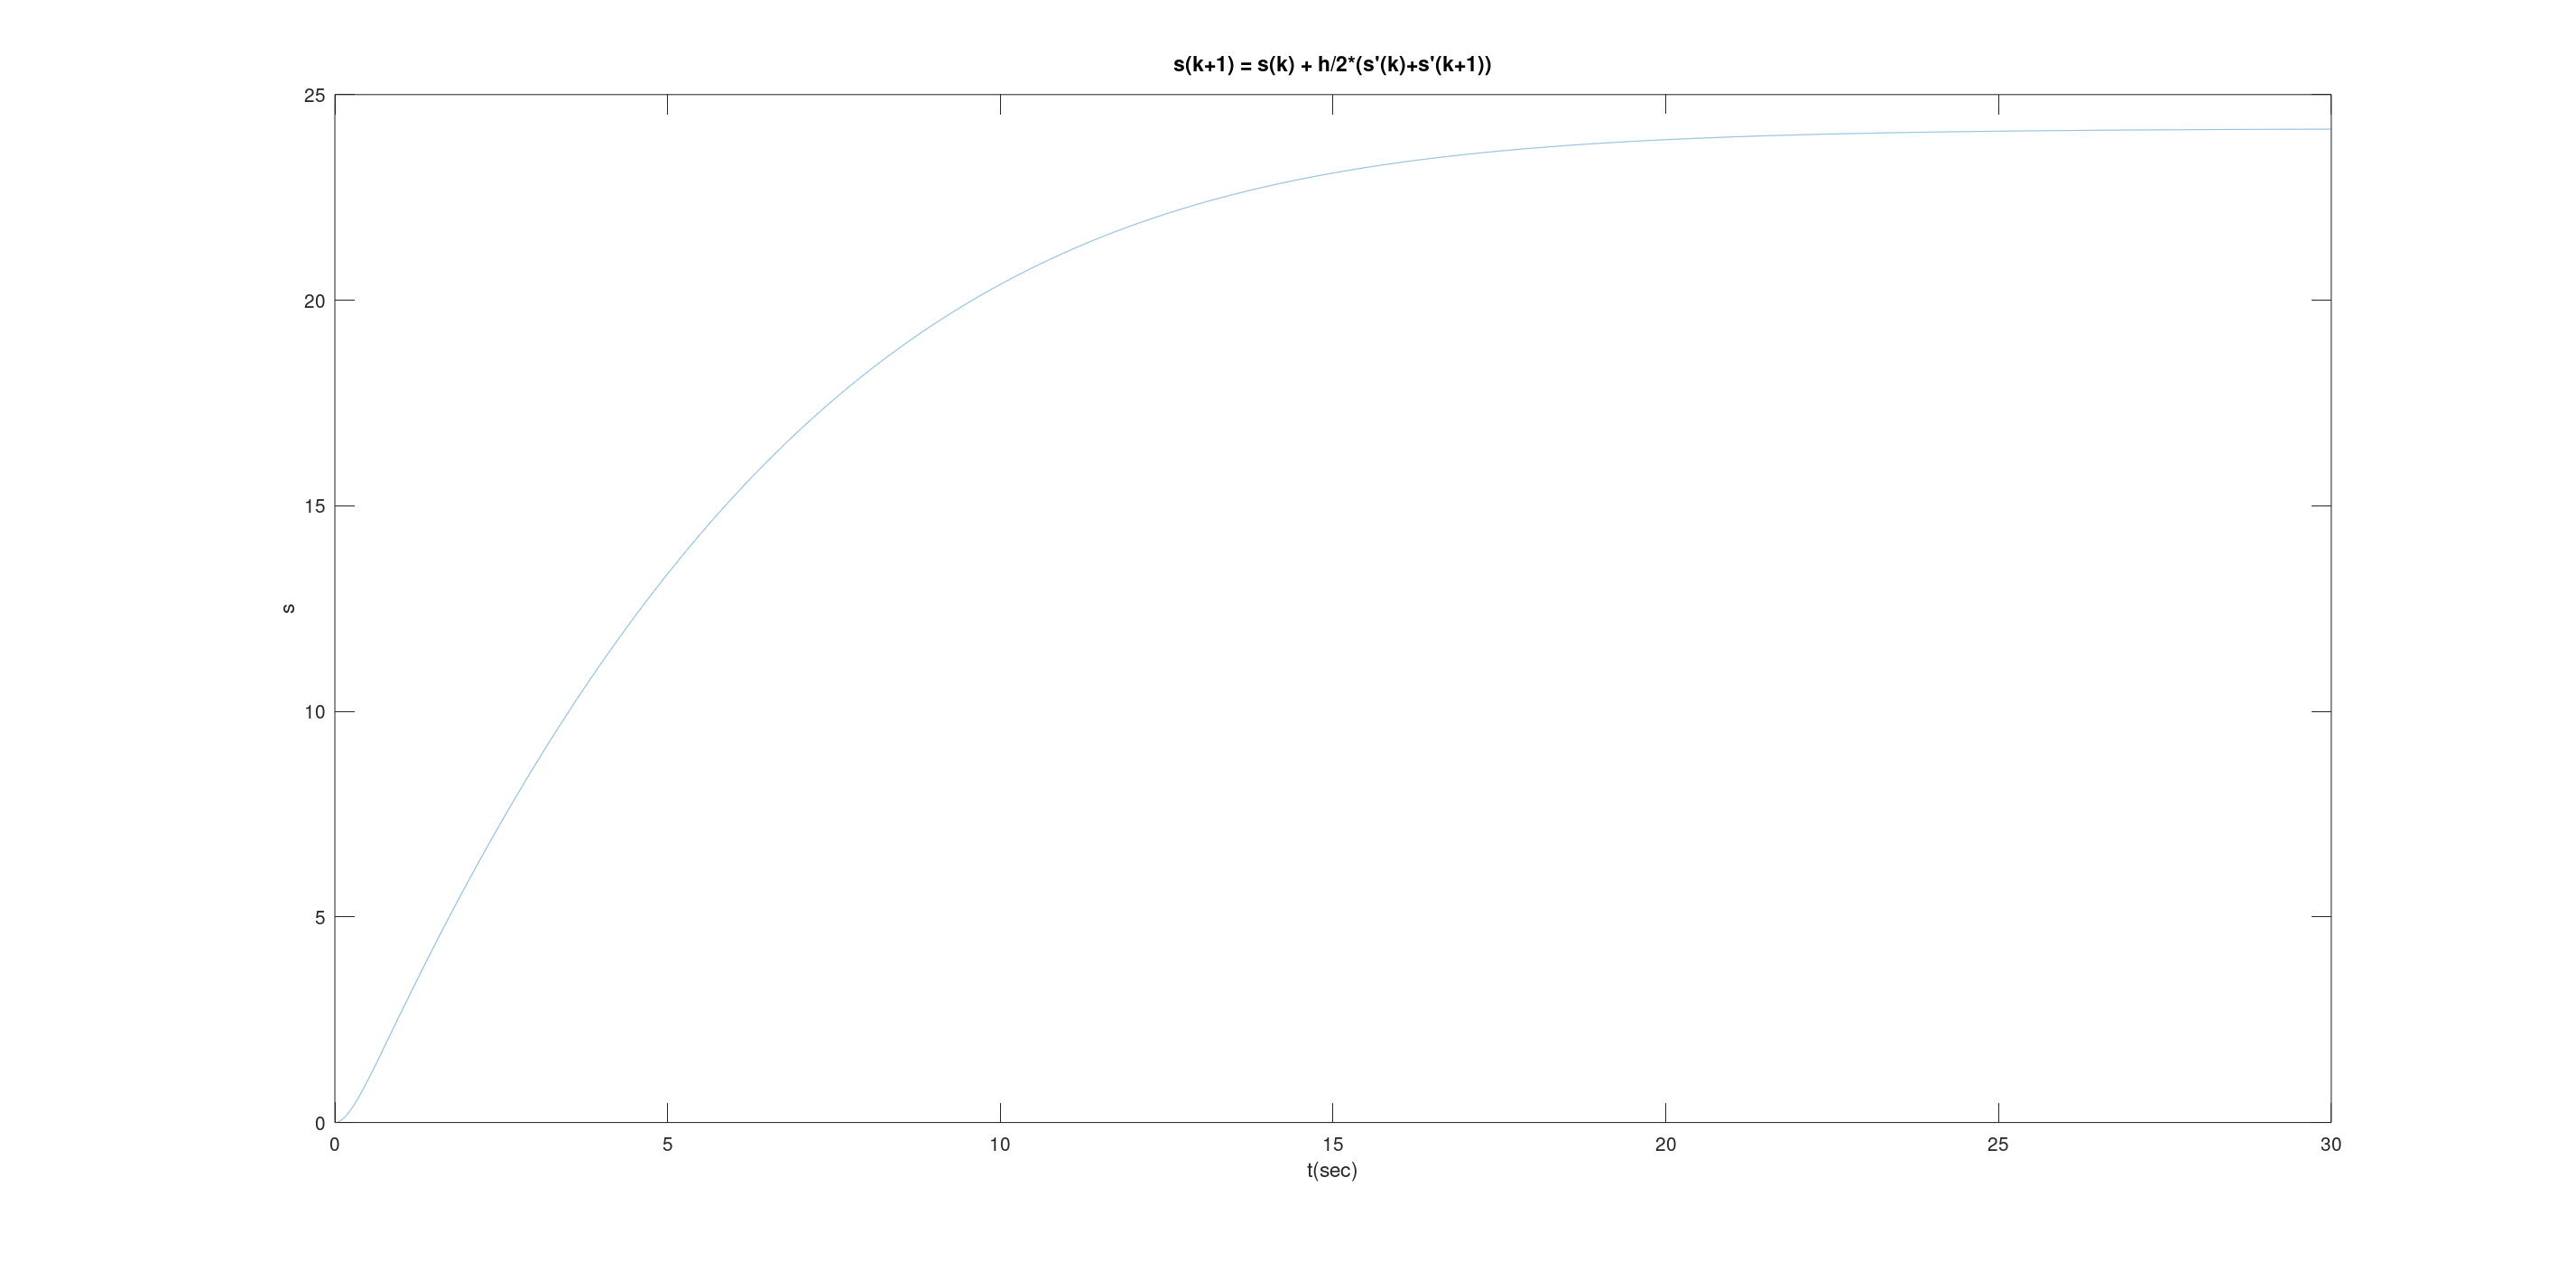
\includegraphics[width=\paperwidth]{problem_1_3_2}}
        \noindent\makebox[\textwidth]{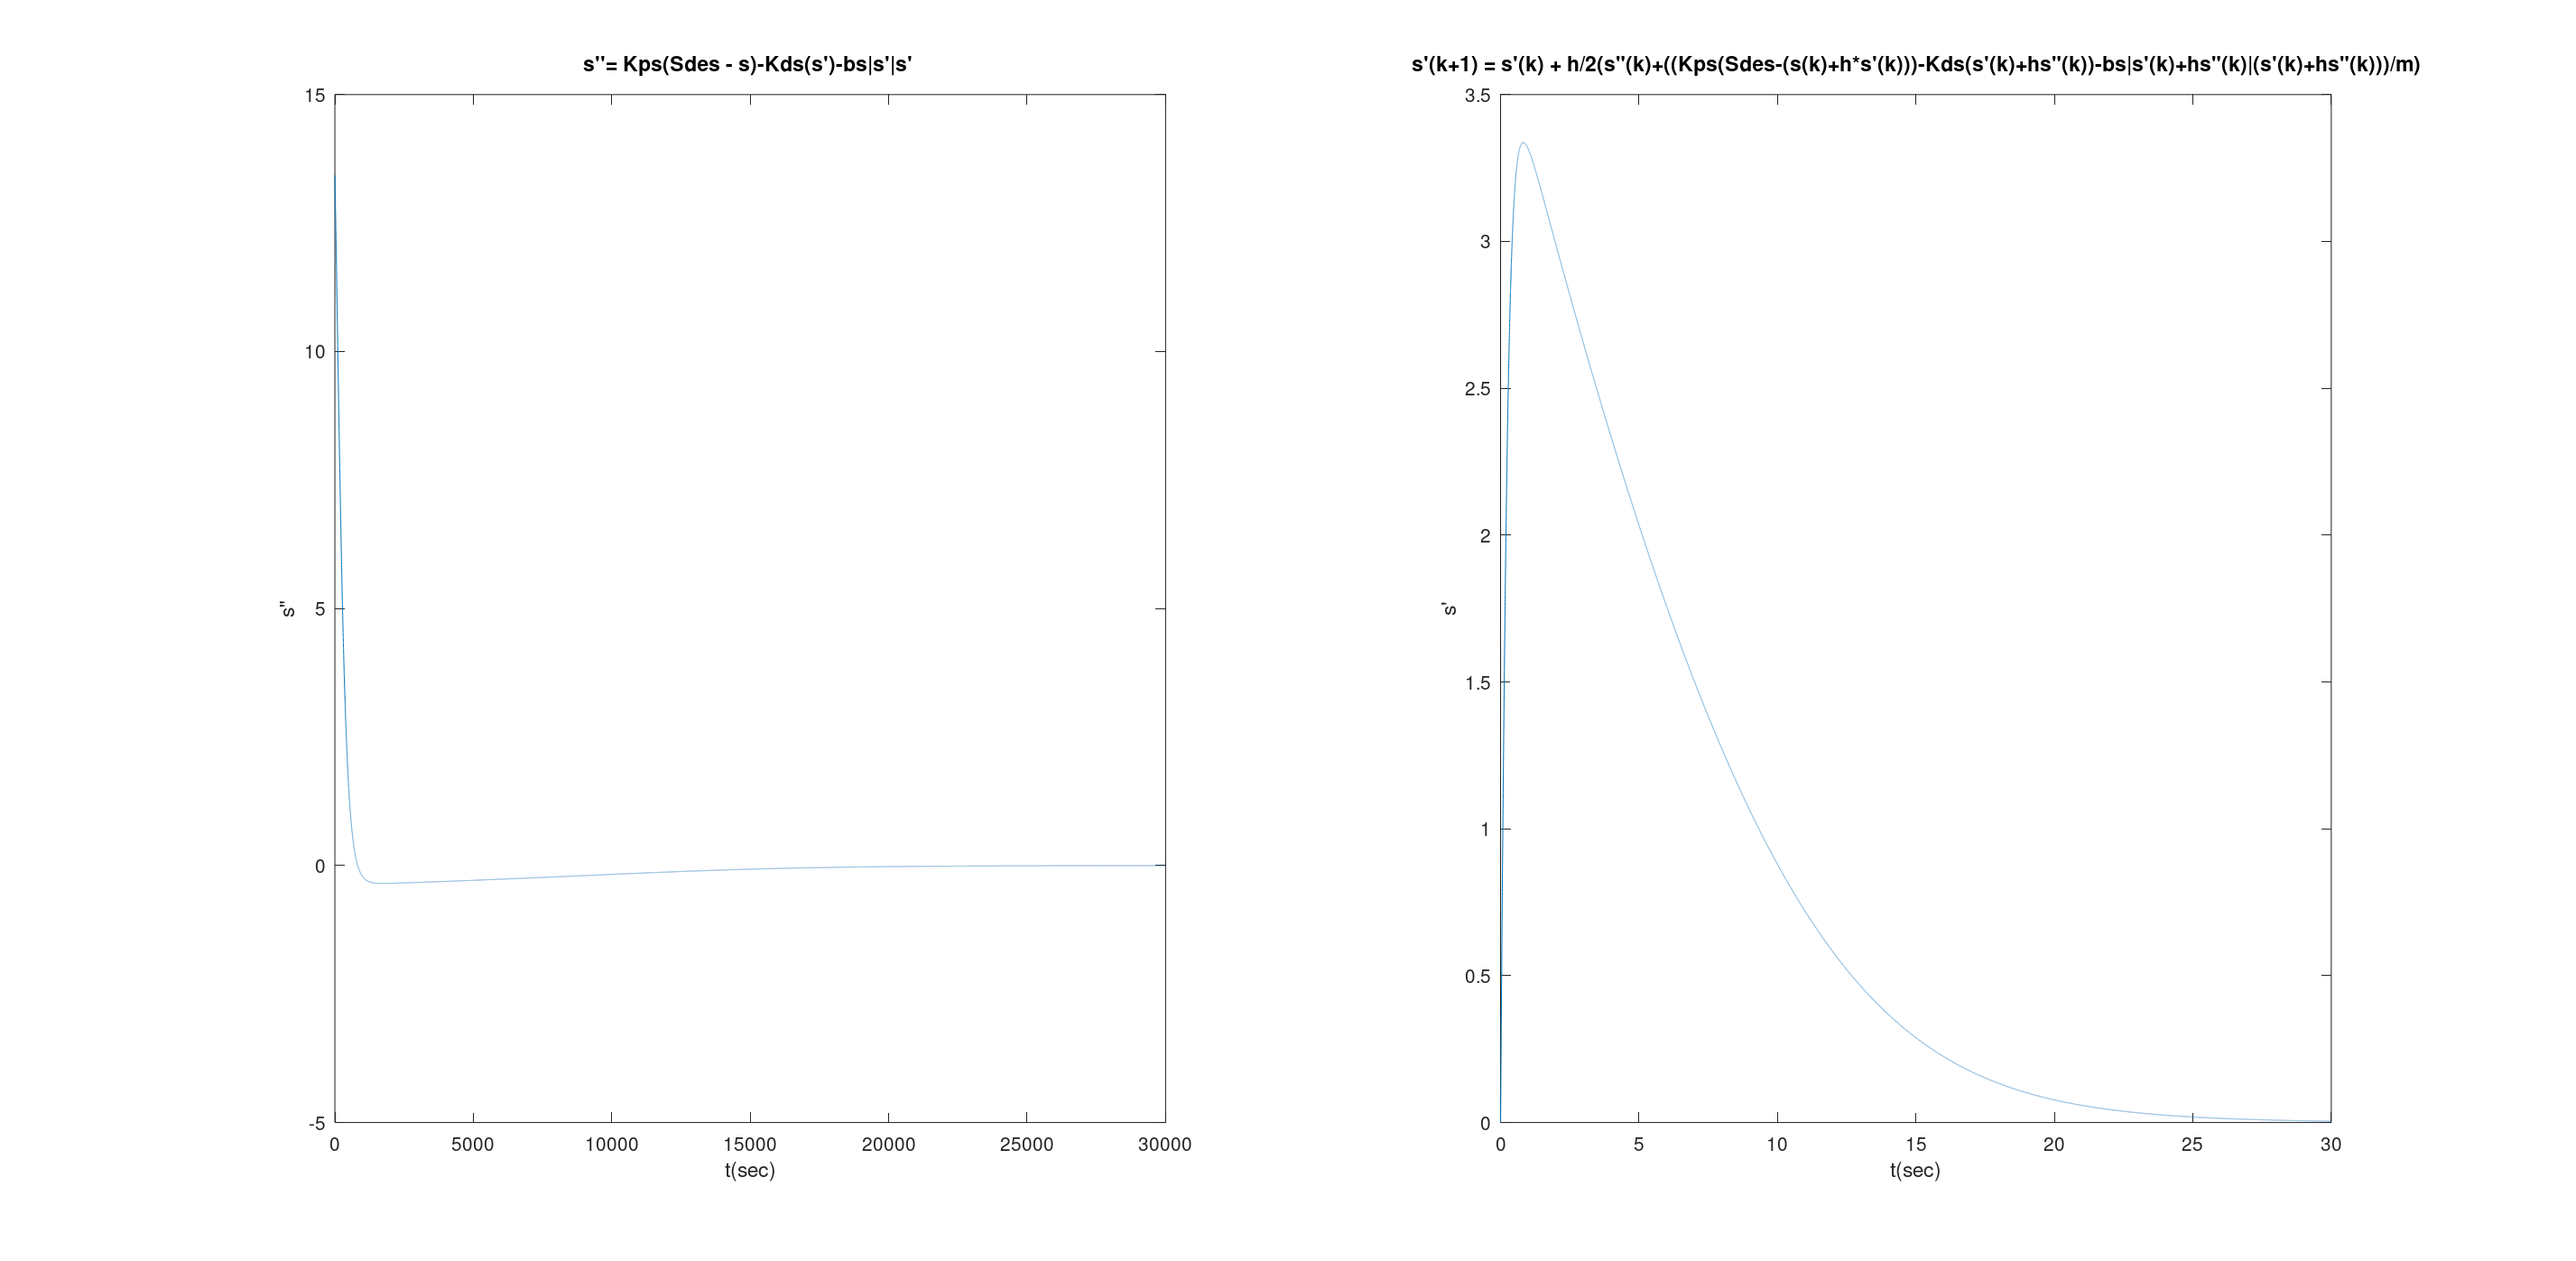
\includegraphics[width=\paperwidth]{problem_1_3_3}}
        \noindent\makebox[\textwidth]{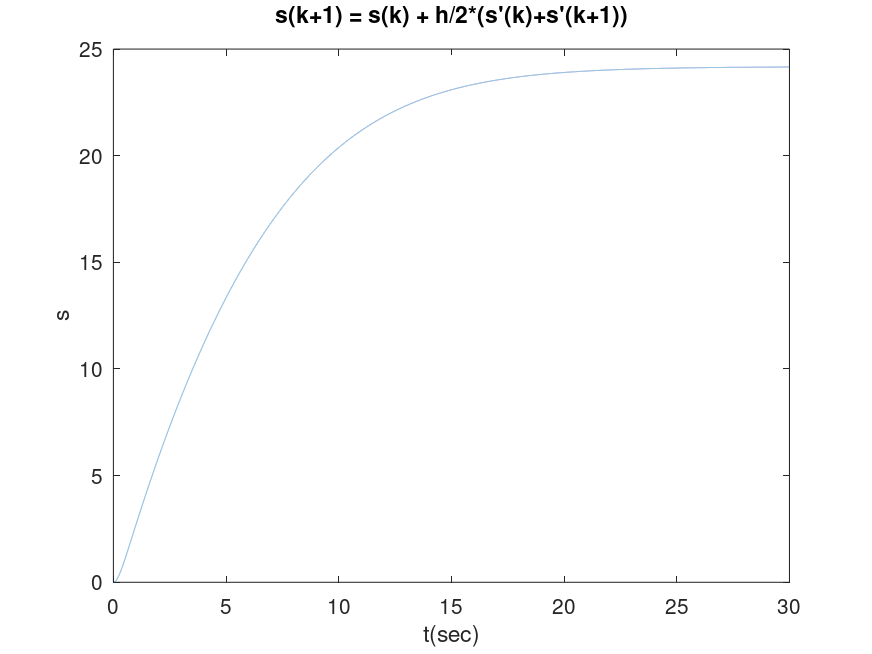
\includegraphics[width=\paperwidth]{problem_1_3_4}}
%-------------------------------------------------------------------------
%-------------------------------------------------------------------------
%-------------------------------------------------------------------------
        \section{Pr'oblhma 2}
        \subsection{Dedom'ena}
        \begin{equation}
            ms''=(f_1+f_2)-b_ss'
            \label{prob2:5}
        \end{equation}
        \begin{equation}
            f_1+f_2=k_{ps}(s_{des}-s)-k_{ds}(s')
            \label{prob2:6}
        \end{equation}
        \subsection{a}
        \[H(s)=\frac{L(output)}{L(input)}\rvert _{A\Sigma=0}\]
        \[a_0y^{(n)}+a_1y^{(n-1)}+\dots a_ny\]
        \[H(s)=\frac{Y(s)}{U(s)}=\frac{1}{a_0s^n+a_1s^{n-1}+\dots+a_n}=\frac{p(s)}{q(s)}\]
        M'ejodos $Laplase$
        \[L(f(t))=f(s)=\int_0^{+\infty}e^{-ts}dt\]
        $f(t)=0$ gia $t<0$
        \[(\ref{prob2:5}) \xRightarrow{(\ref{prob2:6})}K_{ps}(s_{des}-s)-k_{ds}s'=b_s=ms''\]
        \[\Leftrightarrow ms^2X(s)=k_{ps}S_{des}-X(s)k_{ps}-k_{ds}(SX(S))-b_s(sX(s))\]
        \[\Leftrightarrow X(s)=\frac{K_{ps}S_{des}}{ms^2+s(K_{ds}+b_s)+K_{ps}}\]
        \hfill M'ono p'oloi
        \[\frac{X(s)}{S_{des}}=\frac{1}{\frac{ms^2}{k_{ps}}+\frac{s(k_{ds}+b_s)}{k_{ps}}+1}\]
        \[H(s)=\frac{X(s)}{U(s)}=\frac{1}{\frac{ms^2}{k_{ps}}+\frac{s(k_{ds}+b_s)}{k_{ps}}+1}\]\hfill Sun'arthsh metafor'as

        L'unw to polu'wnumo $2_{o\upsilon}$ bajmo'u $\frac{mr^2}{k_{ps}}+s\frac{k_{ds}+b_s}{k_{ps}}+1$ \par
        'Ara oi p'oloi e'inai:
        \[\Delta=(\frac{k_{ds}+b_s}{k_{ps}})^2-4\frac{m}{k_{ps}}\]
        \[r_{1,2}=\frac{-\frac{k_{ds}+b_s}{k_{ps}}\pm \sqrt{\Delta}}{2\frac{m}{k_{ps}}}\]
%-----------------------------------------------------------------------------------------------------------------------------------------------------

        \subsection{g}
        \[ms''=k_{ps}(s_{des}-s)-k_{ds}-s'-b_ss'\]
        \[s''+\frac{s'(k_{ds}-b_s)}{m}+\frac{k_{ps}s}{m}-\frac{k_{ps}s_{des}}{m}=0\]
        \[r^2+\frac{r(k_{ds}+b_s)}{m}+\frac{k_{ps}s}{m}=0\]
        \[\Delta=(\frac{k_{ds}+b_s}{m})^2-4\frac{k_{ps}}{m}\]
        
        \[r_{1,2}=\frac{-\frac{k_{ds}+b_s}{m}\pm\sqrt{\Delta}}{2}\]
        'Ara 'eqoume 2 l'useis, tis $r1$ kai $r2$:
        \[r_1=\frac{-\frac{k_{ds}+b_s}{m}+\sqrt{\Delta}}{2}\]
        \[r_2=\frac{-\frac{k_{ds}+b_s}{m}-\sqrt{\Delta}}{2}\]
        \subsubsection{Merik'h L'ush}
        \[c_1e^{r_1t}+c_2e^{r_2t}=-\frac{k_{ps}s_{des}}{m}\]
        \[s''+s'\frac{k_{ds}+b_s}{m}+\frac{k_{ps}s}{m}-\frac{k_{ps}s_{des}}{m}=0\xRightarrow[s'(0)=0]{s''(0)=0}\]
        \[s''(0)+s'(0)\frac{k_{des}+b_s}{m}+\frac{K_{ps}s(0)}{m}-\frac{k_{ps}s_{des}}{m}=0\Rightarrow\]
        \[s(0)=s_{des}\]
        \[s(t)=s_{des}\]
        $s(t)=s_{des}=A$ 'Ara polu'wnumo $0^{o\upsilon}$ bajmou
        \subsubsection{Genik'h L'ush}
        'Ara,
        \[s=s_{des}+c_1e^{r_1t}+c_2e^{r_2t}\]
        \[s'=c_1r_1e^{r_1t}+c_2r_2e^{r_2t}\]
        \begin{equation}
        s(0)=0\Rightarrow c_1+c_2+s_{des}=0\Rightarrow c_1+c_2=-s_{des}
        \label{eq:s1}
        \end{equation}
        \begin{equation}
            s'(0)=0\Rightarrow c_1r_1e^0+c_2r_2e^0=0\Rightarrow_1r_1+c_2r_2=0
            \label{eq:s2}
        \end{equation}
        \[(\ref{eq:s2})\xRightarrow{(\ref{eq:s1})}(-c_2-s_{des})r_1+c_2r_2=0\Rightarrow_2=\frac{s_{des}r_1}{-r_1+r_2}\]
        \[(\ref{eq:s1})\xRightarrow{(\ref{eq:s2})}c_1=-s_{des}r_1(r_2-r_1)-s_{des}=-s_{des}(\frac{r_1}{r_2-r_1}+1)\]
        \subsubsection{Analutik'h L'ush}
        \[s=s_{des}+(-s_{des}(\frac{r_1}{r_2-r_1}+1))e^(r_1t)+\frac{s_{des}r_1e^{r_2t}}{-r_1+r_2}\]


        \subsection{Eik'ones}
        \subsection{2.g)}
        \noindent\makebox[\textwidth]{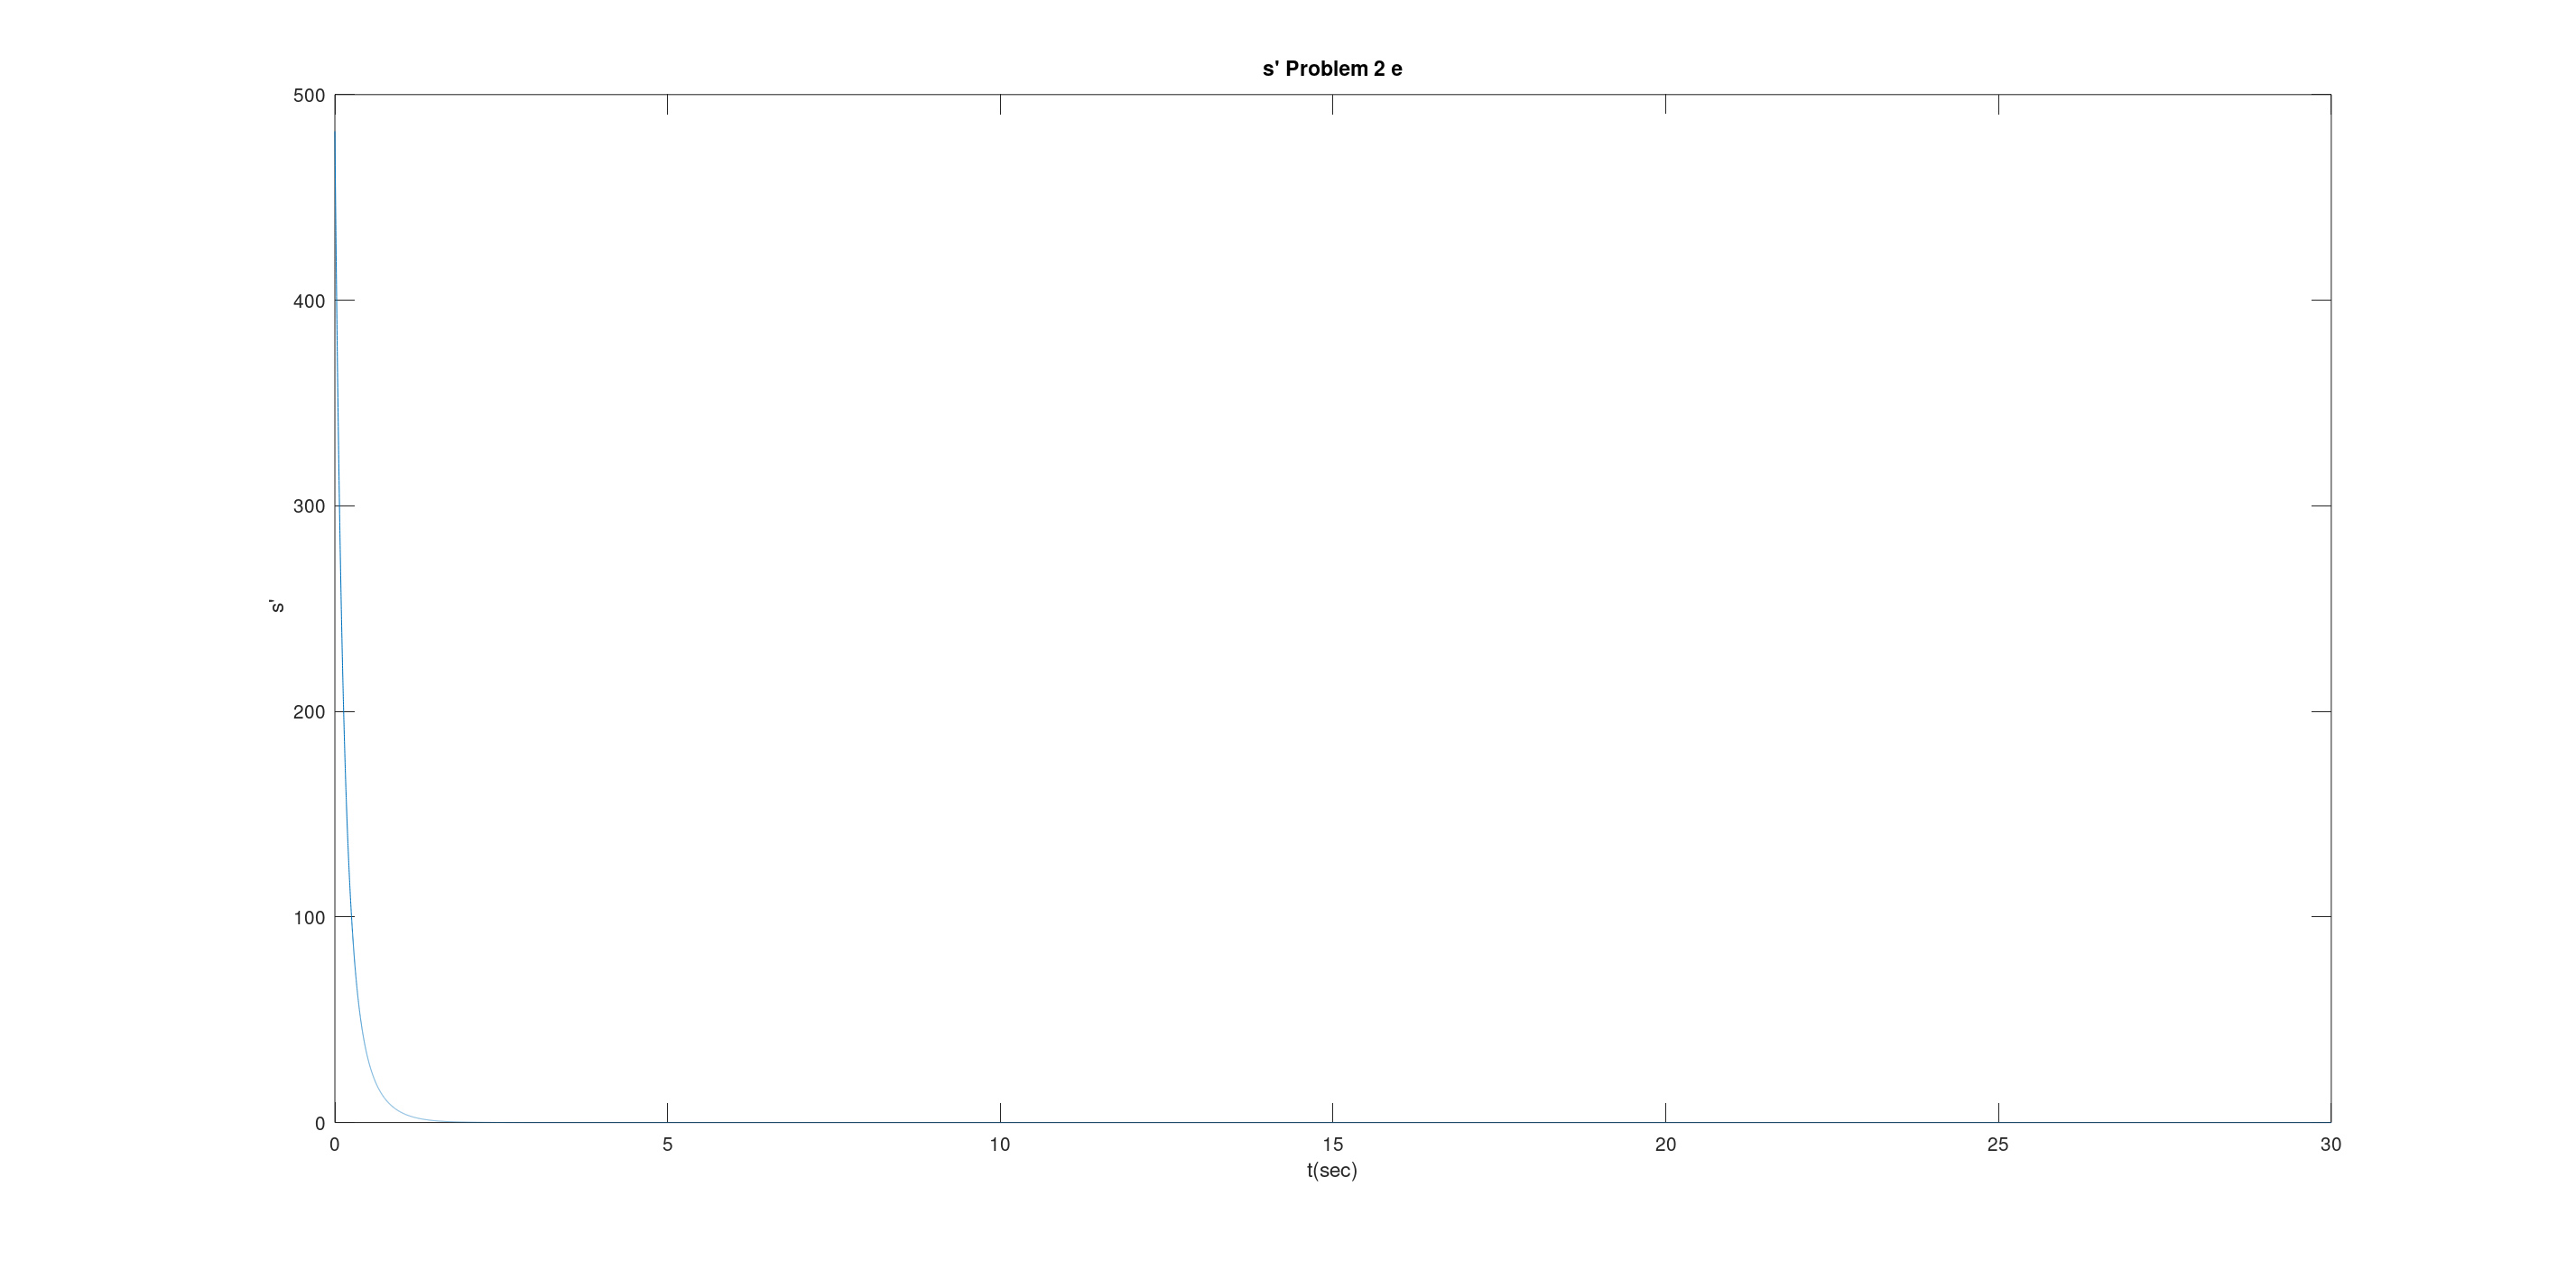
\includegraphics[width=\paperwidth]{problem2d_1}}
        \noindent\makebox[\textwidth]{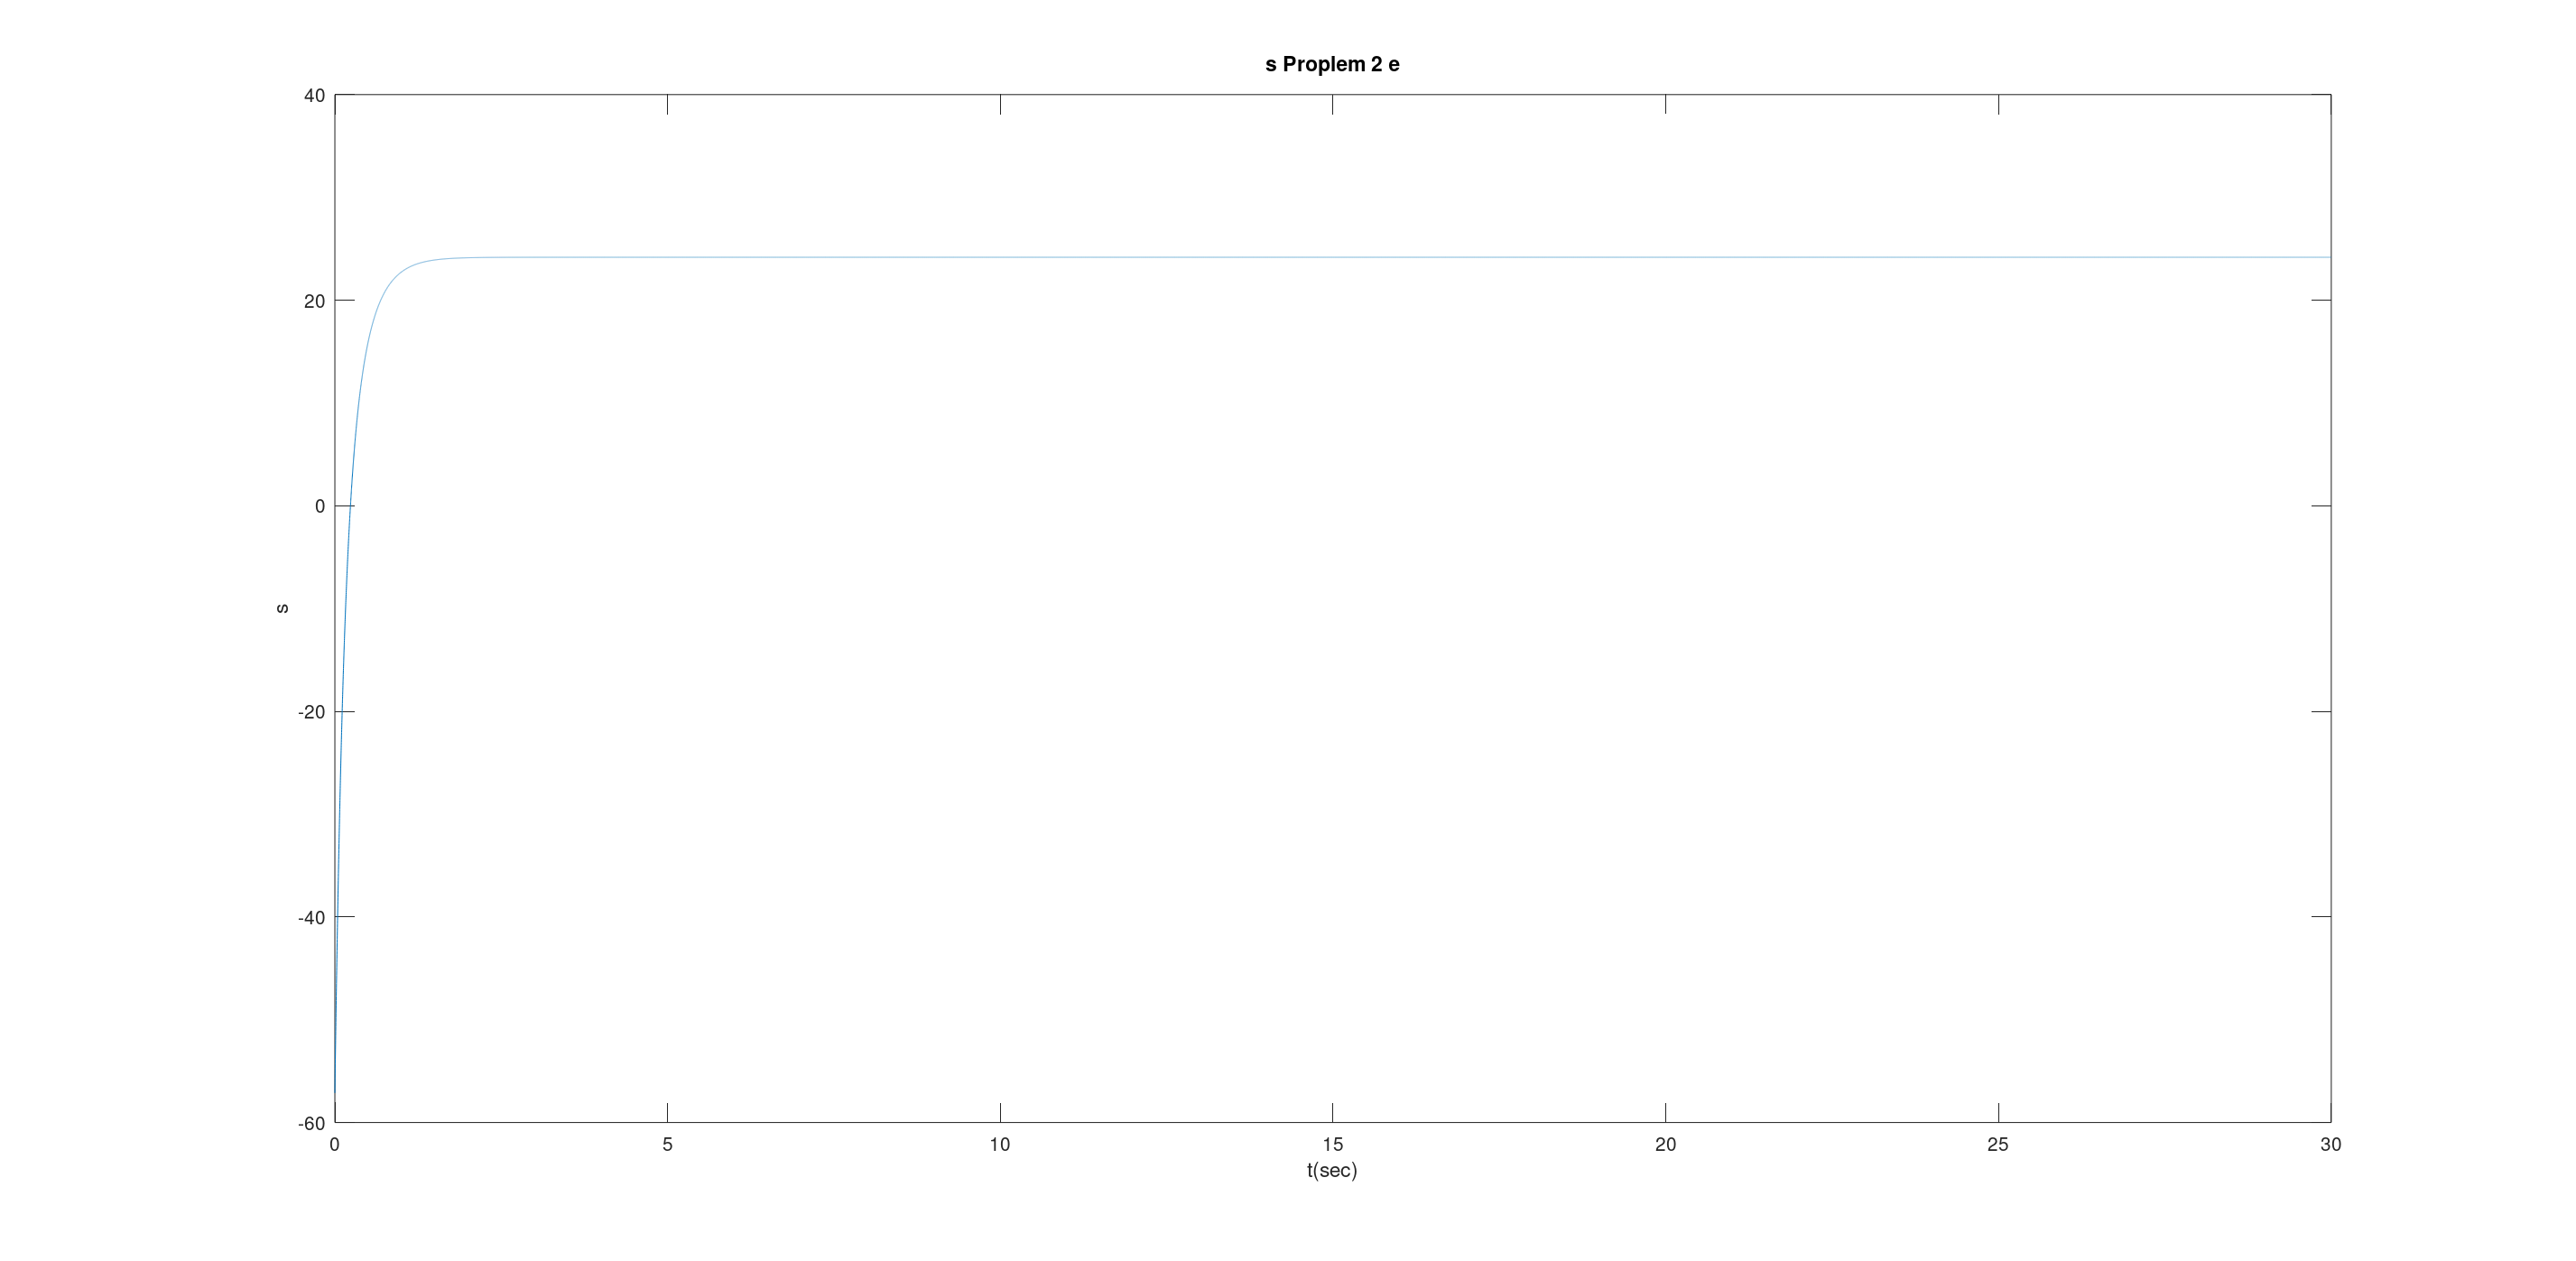
\includegraphics[width=\paperwidth]{problem2d_2}}
\end{document}